\documentclass[class=report,crop=false,border={11pt,10pt}]{standalone}
\usepackage{pacco}
\begin{document}
	\chapter{Exercises and questions}
	\section{Exercises with Prof. Issoglio (2024/2025)}
	\subsection{Exercise class 1}
	\begin{exercise}
		Consider the experiment where we throw a coin infinitely many times, so that 
		\begin{equation*}
			\Omega=\{H,T\}^{\N} \qquad\text{(or $\{0,1\}^{\N}$)}.
		\end{equation*}
		In particular, the event $\omega\in\Omega$ is of the form $\omega=(\omega_1,\omega_2,\ldots)$ with $\omega_i\in\{0,1\}$. Let 
		\begin{equation*}
			C:=\left\{\left\{\omega\in\Omega:\omega_k=a,a\in\{0,1\},n\in\N\right\}\right\}
		\end{equation*}
		and 
		\begin{equation*}
			\F:=\sigma(C).
		\end{equation*}
		We want to check whether $\F$ is a good modeling choice for our experiment. For example, if we set
		\begin{equation*}
			A:=\left\{\omega:\frac{\#\{k\leq n:\omega_k=1\}}{n}\xrightarrow[n\to\infty]{}\frac{1}{2}\right\}
		\end{equation*}
		do we have $A\in\F$?
	\end{exercise}
	Let us introduce a \rv{} (which is a map) $X_n:\Omega\mapsto\R$ given by 
	\begin{equation*}
		X_n=\begin{cases}
			1 &\text{if }\omega_n=1\\
			0&\text{if }\omega_n=0.
		\end{cases}
	\end{equation*}
	Now, $X_n$ is $\F$-measurable (i.e. it is a \rv{} on $(\Omega,\F)$) because for $\every B\in\B(\R)$ we have
	\begin{equation*}
		X^{-1}_{n}(B)=\{\omega\in\Omega:X_n(\omega)\in B\}
	\end{equation*}
	and this set actually belongs to $\F$. Why? Because it basically is
	\begin{equation*}
		\{\omega\in\Omega:X_n(\omega)=B\}=\begin{cases}
			\emptyset&\text{if }0,1\not\in B\\
			\Omega&\text{if }0,1\in B\\
			\{\underbracket{\omega\in\Omega:X_n(\omega)=1}_{{\text{all the $\omega$ with $\omega_n=1$}\implies\in C}}\}&\text{if }0\not\in B,1\in B\\
			\{\underbracket{\omega\in\Omega:X_n(\omega)=0}_{{\text{all the $\omega$ with $\omega_n=0$}\implies\in C}}\}&\text{if }0\in B,1\not\in B\\
		\end{cases}
	\end{equation*}
	So the process is measurable with respect to $\F$: the \sa{} generated by $C$ has all the $\omega$ necessary to fully explain the process. Remember that $B\subset\Omega$! Now let $S_n=\sum_{i=1}^{n}X_i$. Then our set $A$ becomes
	\begin{equation*}
		A=\left\{\omega:\frac{S_n}{n}\xrightarrow[n\to\infty]{}\frac{1}{2}\right\}.
	\end{equation*}We know that $S_n$ is a sum of $\F$-measurable functions and therefore it is $\F$-measurable. We can write $A$ as
	\begin{align*}
		A&=\left\{\omega\in\Omega:\frac{S_n}{n}\to\frac{1}{2}\right\}\\
		&=\left\{\omega\in\Omega:\liminf_{n \to \infty}\frac{S_n}{n}=\limsup_{n\to\infty}\frac{S_n}{n}=\frac{1}{2}\right\}\\
		&=\left\{\underbrace{\omega\in\Omega:\liminf_{n \to \infty}\frac{S_n}{n}=\frac{1}{2}}_{\in\F}\right\}\cap\left\{\underbrace{\omega\in\Omega:\limsup_{n \to \infty}\frac{S_n}{n}=\frac{1}{2}}_{\in\F}\right\}
	\end{align*}
	since $S_n$ is $\F$-measurable, so are its $\limsup$ and $\liminf$. By doing so we went from the limit, which is not a nice thing to handle when it comes to measurability, to $\liminf$ and $\limsup$ that are more manageable objects.
	\begin{exercise}
		Let $\Omega=\{0,1\}^{\N}$. For a given $n\in\N$ let 
		\begin{equation*}
			\mathcal{A}_n=\left\{\{\omega=(\omega_1,\omega_2,\cdots)\in\Omega:(\omega_1,\ldots,\omega_n)\in B\}\text{for some }B\subset\{0,1\}^{n}\right\}.
		\end{equation*}
		\begin{enumerate}[\circnum]
			\item Show that $\mathcal{A}_n$ is a \sa.
			\item Show that $\bigcup_{n\in\N}\mathcal{A}_{n}$ is not a \sa.
		\end{enumerate}
	\end{exercise}
	\begin{enumerate}[\circnum]
		\item If we show that $\mathcal{A}_n$ is finite, then it is enough to prove that it is an algebra, since the closure under \textit{union, intersection and complementation} will automatically follow from this.\\
		We easily see that $\mathcal{A}_n$ is finite because $n$ is fixed so $\{0,1\}^{n}$ is finite and since the varying set in this case is $B\subset\{0,1\}^{n}$ then also $\mathcal{A}_n$ must be finite. For example we would get
		\begin{equation*}
			\mathcal{A}_1=\left\{\{\omega\in\Omega:\omega_1\in\{0\}\},\{\omega\in\Omega:\omega_1\in\{1\}\},\{\omega\in\Omega:\omega_1\in\{0,1\}\},\{\omega\in\Omega:\omega_1\in\emptyset\}\right\}.
		\end{equation*}
		We can also check that this is an algebra:
		\begin{enumerate}
			\item it is obvious that $\emptyset\in\mathcal{A}_n$;
			\item let $A\in\mathcal{A}_n$. This means that $\exists B\subset\{0,1\}^{n}$ such that
			\begin{equation*}
				A=\{\omega\in\Omega:(\omega_1,\ldots,\omega_n)\in B\}
			\end{equation*}
			and so
			\begin{align*}
				A^c&=\{\omega\in\Omega:(\omega_1,\ldots,\omega_n)\notin B\}
			\end{align*}
		\end{enumerate}
	\end{enumerate}
	\subsection{Exercise class 2}
	\subsection{Exercise class 3}
	\subsection{Exercise class 4}
	\subsection{Exercise class 5}
	\subsection{Exercise class 6}
	\subsection{Exercise class 7}
	\subsection{Exercise class 8}
	\section{Questions for the oral examination}
	Here I will try and answer to the questions that were on the moodle site about the year 2022-2023. I hope that they will be valid for the years to come as well.
	\subsection{Transition kernels: definition, example, and their usage in the extension of measures to
		product spaces}
	First of all, the definition:
	\begin{definition}
		Let $(E,\E)$ and $(F,\F)$ be measurable spaces. Let $K$ be a mapping from $E\times\F$ into $\overline{\R}_+$. Then $K$ is called \emph{transition kernel} from space $(E,\E)$ into space $(F,\F)$ if:
		\begin{itemize}
			\item the mapping $x\mapsto K(x,B)$ is $\E$-measurable $\every B\in\F$;
			\item the mapping $B\mapsto K(x,B)$ (the second mapping of the kernel, the one regarding the set) is a measure $\every x\in E$.
		\end{itemize}
	\end{definition}
	Then the example:
	\begin{example}
		Take $\nu$, a finite measure on $(F,\F)$ and take $k$, a positive function on $(E\times F)$ which is measurable with respect to $\E\otimes\F$, the product \sa{}. Then, we integrate
		\[\int_B\nu(\dy)k(x,y)\qquad\begin{array}{l}
			B\in\F\\
			x\in E
		\end{array}\]
		We see how this object depends on $x$ and on the choice of $B$ (a function of $x$ and $B$...). It defines a transition kernel
		\[K(x,B)=\int_B\nu(\dy)k(x,y)\qquad\begin{array}{l}
			B\in\F\\
			x\in E
		\end{array}\]
		from $(E,\E)$ into $(F,|F)$.
	\end{example}
	Now the extensions of measures on product spaces;
	\begin{theorem}
		\emph{Extension of measures on product spaces}.\\
		Let $\mu$ be a measure on the measurable space $(E,\E)$. Let $K$ be a $\Sigma$-finite\footnote{Erm... what the sigma?} transition kernel from space $(E,\E)$ into $(F,\F)$. Then:
		\begin{enumerate}[\circnum]
			\item if we take our function $f(x,y)$, integrate it against our kernel $K(x,\dx)$ over $F$ and then integrate again against measure $\mu$ over $E$, the operation 
			\[\pi f=\int_E\mu(\dx)\int_FK(x,\dy)f(x,y)\]
			defines a measure $\pi$ on $(E\times F,\E\otimes\F)$;
			\item if $\mu$ is $\sigma$-finite and $K$ is $\sigma$-bounded then $\pi$ is $\sigma$-finite and it is the unique measure on $(E\times F,\E\otimes\F)$ satisfying
			\[\pi(A\times B)=\int_A\mu(\dx)K(x,B)\qquad\every A\in\E,B,\in\F.\]
		\end{enumerate}
	\end{theorem}
	\subsection{Kolmogorov’s 0-1 law: proof and an example of its usage}
	First, the statemente of the theorem.
	\begin{theorem}
		\emph{Kolmogorov's 0-1 law}\\
		This is a theorem about independence. Let $\G_1,\G_2,\ldots$ be independent. Then
		\[\pr(H)=\begin{cases}
			0\\
			1
		\end{cases}\qquad\every H\in\tau.\]
	\end{theorem}
	and here's the short proof:
	\begin{fancyproof}
		Start from your independency $(\G_1,\G_2,\ldots)$, then put the last $\G$'s in a partition (which is still an independency) $(\G_1,\G_2,\ldots,\G_n,\tau_n)$. Now consider that the tail \sa{} is a subset of $\tau_n$ and this means that $(\G_1,\G_2,\ldots,\G_n,\tau)$ is still an independency... But we also know that this is true for every $n$ up to $\infty$ and so we can extend the independency to a collection of countably many partitions, since ${(\G_1,\G_2,\ldots,\G_n,\tau)}_{n}$ us a countably infinite sequence of independencies. So
		\begin{equation*}
			(\tau,\G_1,\G_2,\ldots)
		\end{equation*}
		is an independency. Do another partition (which still gives us an independency) and get the independency
		\begin{equation*}
			(\tau,\tau_0)
		\end{equation*}
		but then remember that $\tau_0$ is an \textit{union} of the \sa s from 1 to $\infty$ while $\tau$ is an \textit{intersection} of all $\tau_n$ including $\tau_0$, so we have that $\tau\subset\tau_0$.\\
		Consider now $\pr(H\cap G)$ where $H\in\tau$ and $G\in\tau_0$. Due do independency we have that 
		\begin{equation*}
			\pr(H\cap G)=\pr(H)\pr(G)
		\end{equation*}but since all elements of $\tau$ are also elements of $\tau_0$ we can choose $G\equiv H$ and our equation becomes
		\begin{equation*}
			\pr(H\cap G)=\pr(H\cap H)=\pr(H)=\pr(H)^{2}
		\end{equation*}
		and the solution to this can only be 0 or 1.
	\end{fancyproof}
	We still need an example of the application... that would be, for example, the behavior in the limits of a sequence of \rv s with independence between $\{X_{n}\}$. Then if the limit exists it is a constant, since $\lim_{n}X_{n}$ belongs to the tail \sa{} of the sequence. Independency between \rv s tells us that we can apply Kolmogorov's 0-1 law to say that $\pr(\lim_{n}X_{n}=\infty)$ is either 0 or 1... but if we somehow know that the limit exists then it can't be $\infty$ so its probability of being $\infty$ is 0 and therefore it is a constant almost surely! This is cool because it tells us that the limit is either infinite or finite. This is useful for sub-martingales. 
	\subsection{Almost sure convergence: definition, properties and characterization theorem}
	Start with the definition:
	\begin{definition}
		A real-valued sequence of \rv s ${(X_n)}_{n}$ on $(\Omega,\HS,\pr)$ is said to be \emph{almost sure convergent} (a.s. convergent) is the numerical sequence
		\[{\Big(X_n(\omega)\Big)}_{n}\]
		converges for almost all $\omega\in\Omega$. \\
		It is said to converge to $X$ if $X$ is an almost sure real-valued \rv{} and 
		\[\lim_{n\to\infty}X_n(\omega)=X(\omega)\]
		for almost all $\omega\in\Omega$.
	\end{definition}
	The characterization is
	\begin{theorem}
		\emph{Characterization of almost sure convergence}:\\
		A sequence of real valued \rv s ${(X_n)}_{n}$ converges to $X$ almost surely \ifonly{}, for every $\varepsilon>0$,
		\begin{equation*}
			\sum_n\mathcal{i}_\varepsilon\circ|X_n-X|<\infty
		\end{equation*}
		almost surely.
	\end{theorem} Where $\mathcal{i}_\varepsilon$  is the indicator function of $(\varepsilon,\infty)$:
	\[\mathcal{i}_\varepsilon(x)=\indi_{(\varepsilon,\infty)}(x)=\begin{cases}
		1, &x>\varepsilon\\
		0, &x\leq \varepsilon.
	\end{cases}\]
	This basically means that in every interval from a certain point $\varepsilon$ to $\infty$ the sum of the differences of $X_n$ and $X$ must not diverge. Here are some properties:
	\begin{itemize}
		\item \textbf{Comparison with Other Types of Convergence:}
		\begin{itemize}
			\item If $\{X_n\}$ converges almost surely to $X$, then $\{X_n\}$ also converges to $X$ in probability.
			\item Almost sure convergence implies convergence in distribution, but not necessarily vice versa.
		\end{itemize}
		
		\item \textbf{Closure Under Linear Operations:}
		\begin{itemize}
			\item \textbf{Addition:} If $X_n \to X$ a.s. and $Y_n \to Y$ a.s., then $X_n + Y_n \to X + Y$ a.s.
			\item \textbf{Multiplication:} If $X_n \to X$ a.s. and $Y_n \to Y$ a.s., then $X_n Y_n \to XY$ a.s. (provided $X$ and $Y$ are bounded or measurable in a compatible way).
		\end{itemize}
		
		\item \textbf{Countable Additivity:}
		\begin{itemize}
			\item \textbf{Countable Unions:} If $\{X_n\}$ converges almost surely to $X$, then for any countable collection of events $\{A_i\}$ with $\Pr(A_i) \to 0$, $\Pr(\limsup_{i \to \infty} A_i) = 0$.
		\end{itemize}
		
		\item \textbf{Uniform Integrability:}
		\begin{itemize}
			\item \textbf{Expectation Convergence:} If $\{X_n\}$ converges almost surely to $X$ and $\{X_n\}$ is uniformly integrable, then $X_n \to X$ in $L^1$, meaning $\mathbb{E}[|X_n - X|] \to 0$.
		\end{itemize}
		
		\item \textbf{Continuity from Below and Above:}
		\begin{itemize}
			\item \textbf{From Below:} If $X_n \leq X_{n+1}$ a.s. for all $n$ and $X_n \to X$ a.s., then $X_n \leq X$ a.s.
			\item \textbf{From Above:} If $X_n \geq X_{n+1}$ a.s. for all $n$ and $X_n \to X$ a.s., then $X_n \geq X$ a.s.
		\end{itemize}
		
		\item \textbf{Interchange of Limits:}
		\begin{itemize}
			\item \textbf{Expectation Limit:} If $X_n \to X$ a.s. and $\{X_n\}$ is uniformly integrable, then $\mathbb{E}[X_n] \to \mathbb{E}[X]$.
		\end{itemize}
		
		\item \textbf{Fatou's Lemma and Monotone Convergence Theorem:}
		\begin{itemize}
			\item \textbf{Fatou’s Lemma:} If $X_n \geq 0$ almost surely and $X_n \to X$ a.s., then $\mathbb{E}[X] \leq \liminf_{n \to \infty} \mathbb{E}[X_n]$.
			\item \textbf{Monotone Convergence Theorem (for non-negative random variables):} If $X_n \to X$ a.s. and $X_n \geq 0$ a.s., then $\mathbb{E}[X] = \lim_{n \to \infty} \mathbb{E}[X_n]$.
		\end{itemize}
	\end{itemize}
	\subsection{Borel Cantelli lemmas; proof of the divergence part}
	Enunciate the two lemmas side by side (and with a slightly different formulation).
	\begin{theorem}
		\emph{Borel-Cantelli lemmas}\\
		\begin{enumerate}[a)]
			\item Let ${(B_n)}_{n}$ be a sequence of Bernoulli \rv s.
			\[\sum_n \ev B_n<+\infty\implies\sum_n B_n<+\infty\as\]
			\item If 
			\[\sum_n\ev B_n=\infty\text{ and }{(B_n)}_{n}\text{ are pairwise independent}\]
			then
			\[\sum_n B_n=+\infty\as\]
		\end{enumerate}
	\end{theorem}
	Now let's prove the divergent part.
	\begin{notation}
		\[p_n=\ev B_n,\quad a_n=\sum_{i=1}^n\ev B_i=\sum_{i=1}^{n}p_i\]
		and we get the partial sum and the limits
		\[S_n=\sum_{i=1}^{n}B_i,\quad S=\lim_n S_n\]
	\end{notation}
	\begin{fancyproof}
		Ok, this is long. We know that, since the \rv s are pairwise independent,
		\begin{equation*}
			\var S_{n}=\sum_{i=1}^{n} \var B_{n}=\sum_{i=1}^{n} p_{n}(1-p_{n})\leq\sum_{i=1}^{n}p_n=a_{n}.
		\end{equation*}
		Then fix $b\in(0,\infty)$. Since we know that ${(a_{n})}_{n}$ is increasing towards $\infty$ then the same can be said of 
		\begin{equation*}
			{\left(a_{n}-\sqrt{ba_{n}}\right)}_{n}
		\end{equation*}
		since we are subtracting to $a_{n}$ a quantity that goes towards $\infty$ more slowly. So the sequence still goes towards infinity and this means that the event ${S<\infty}$ is basically the limit of the increasing sequence of events 
		\[{\left\{S<a_{n}-\sqrt{ba_{n}}\right\}}_{n}.\]
		Since $S_{n\leq S}$ we have that
		\begin{equation*}
			\left\{S<a_{n}-\sqrt{ba_{n}}\right\}\subset\left\{S_{n}<a_{n}-\sqrt{ba_{n}}\right\}
		\end{equation*}
		and we also have that
		\begin{equation*}
			\left\{S_{n}<a_{n}-\sqrt{ba_{n}}\right\}\subset\left\{|S_{n}-a_{n}|>\sqrt{ba_{n}}\right\}
		\end{equation*}
		Since we are dealing with inclusion of events we can look at this from the point of view of probability measures:
		\begin{equation*}
			\pr\left(S<a_{n}-\sqrt{ba_{n}}\right)\leq\pr\left(S_{n}<a_{n}-\sqrt{ba_{n}}\right)\leq\pr\left(|S_{n}-a_{n}|>\sqrt{ba_{n}}\right).
		\end{equation*}
		We take the $\limsup_n$ for two of these probabilities:
		\begin{equation*}
			\limsup_n\left(\pr\left(S<a_{n}-\sqrt{ba_{n}}\right)\right)\leq\limsup_n\left(\pr\left(|S_{n}-a_{n}|>\sqrt{ba_{n}}\right)\right)
		\end{equation*}
		but the first term of this inequality becomes
		\begin{align*}
			\limsup_n\left(\pr\left(S<a_{n}-\sqrt{ba_{n}}\right)\right)&=\pr\left(\lim_{n}\left(\pr\left(S<a_{n}-\sqrt{ba_{n}}\right)\right)\right)\\
			&=\pr\left(S<\infty\right)
		\end{align*}
		since the quantity ${\left\{S<a_{n}-\sqrt{ba_{n}}\right\}}_{n}$ goes towards infinity. Now we can rewrite the previous inequality and use Chebyshev's inequality:
		\begin{align*}
			\pr\left(S<\infty\right)&\leq\limsup_n\left(\pr\left(|S_{n}-a_{n}|>\sqrt{ba_{n}}\right)\right)\\
			&\leq\limsup_n\left(\frac{\var S_{n}}{ba_{n}}\right)\\
			&\leq\limsup_n\left(\frac{\cancel{a_{n}}}{b\cancel{a_{n}}}\right)=\frac{1}{b}.
		\end{align*}
		Since $b$ is arbitrary we can let it go towards infinty and thus obtain that
		\begin{equation*}
			\pr\left(S<\infty\right)\leq0
		\end{equation*}
		But this means that the probability of the complementary event must be 1:
		\begin{equation*}
			\pr\left(S=\infty\right)=1.
		\end{equation*}
	\end{fancyproof}
	\subsection{Borel Cantelli lemmas; proof of the convergence part, relations with a.s. convergence and
		examples of its application}
	Start by enunciating the theorem.
	\begin{theorem}
		\emph{First Borel-Cantelli Lemma}
		Let ${(H_n)}_{n}$ be a sequence of events. Then
		\[\sum_n\pr(H_n)<+\infty\implies\sum_n\indi_{H_n}<+\infty\quad\text{a.s.}\]
	\end{theorem}
	The proof is no shit:
	\begin{fancyproof}
		Denote $N=\sum\indi_{H_{n}}$ so that $\sum_{n}\pr(H_{n})=\sum_n\ev\indi_{H_{n}}=\ev\sum\indi_{H_{n}}=\ev N$. This means that the new claim is
		\begin{center}
			``If $\ev N<\infty$ then $N<\infty$''
		\end{center}
		But this is true because if the expectation is finite so is its \rv{}. Of course almost surely...
	\end{fancyproof}
	Now the implications for a.s. convergence:
	\begin{proposition}
		Let
		\[\sum_n\pr(|X_n-X|>\varepsilon)<+\infty\qquad\every\varepsilon>0.\]
		Then 
		\[X_n\xrightarrow[]{\text{a.s.}}X.\]
	\end{proposition}
	\begin{proposition}
		Suppose that there exists a sequence ${(\varepsilon_n)}_{n}$ decreasing to 0 such that
		\[\sum_n\pr(|X_n-X|>\varepsilon_n)<+\infty.\]
		Then
		\[X_n\convas X.\]
	\end{proposition}
	So we don't need $\varepsilon$ to be constant, but just to be decreasing to 0.
	\begin{proposition}
		Suppose that there exists a sequence of positive numbers ${(\varepsilon_n)}_{n}$ such that
		\[\sum_n\varepsilon_n<+\infty,\quad\sum_n\pr(|X_{n+1}-X_n|>\varepsilon_n)<+\infty\]
		Then $X_n$ converges almost surely.
	\end{proposition}
	\subsection{Convergence in probability: definition, properties and theorem on the metric for
		convergence in probability}
	Let's start with the definition:
	\begin{definition}
		Let ${(X_n)}_{n}$ be a sequence of real-valued random variables. Then ${(X_n)}_{n}$ converges to a further real-valued \rv{} \emph{in probability} if 
		\[\lim_n\pr(|X_n-X|>\varepsilon)=0\qquad\every\varepsilon>0.\]
	\end{definition}
	I am not sure about properties, why can't you state things clearly? Fuck off. 
	\begin{theorem}
		\emph{Characterization theorem for convergence in probability}. 
		\begin{enumerate}[label=\textit{\roman*})]
			\item \label{ehehe} if ${(X_n)}_{n}$ converges to $X$ almost surely, then it converges to $X$ in probability;
			\item \label{ehehe2} if ${(X_n)}_{n}$ converges in probability to $X$, then it has a subsequence converging to the same \rv{} $X$ almost surely;
			\item \label{ehehe3} if every subsequence of the main sequence has a further subsequence converging to $X$ almost surely, then the main sequence converges to $X$ in probability.
		\end{enumerate}
	\end{theorem}
	\begin{remark}
		Convergence in probability is preserved under arithmetic operations. 
	\end{remark}
	So, for example if we have $X\convpr X$ and $Y_n\convpr Y$ then ${(X_n+Y_n)}_{n}\convpr X+Y$.\\
	We will now introduce a metric for convergence in probability: since we are talking about \textit{distance}, we may think\footnote{A remark that reeks of overestimation.} that this has something to do with \textit{metric spaces}, where we measure the distance between different objects. Indeed there is a connection between measure spaces and metric spaces...\par
	Let us introduce now a metric for convergence in probability. If we want to calculate a metric between \rv s $X$ and $Y$ we can define the following metric:
	\[d(X,Y)=\ev(|X-Y|\wedge1).\]
	\begin{remark}
		\begin{enumerate}[\circnum]
			\item $d(X,Y)=0 \iff X=Y\as$
			\item $d(X,Y)+d(Y,Z)\geq d(X,Z).$
		\end{enumerate}
		$d$ is a metric on the space of real-valued \rv s if $X$ and $Y$ are indentified as the same \rv{} if $X=Y$ almost surely.
	\end{remark}
	\begin{proposition}
		\[ X_n\convpr X\iff d(X_n,X)\xrightarrow[n\to\infty]{}0. \]
	\end{proposition}
	\subsection{Uniform integrability: definitions and its consequences}
	Start with the definition
	\begin{definition}
		A collection of random variables K is said to be \emph{uniformly integrable} if
		\[k(b)=\sup_{X\in K}\left(\ev|X|\indi_{(|X|>b)}\right)\]
		goes to 0 as $b\to\infty$. 
	\end{definition}
	What about the properties?
	\begin{enumerate}[\circnum]
		\item If $K$ is finite and each $X\in K$ is integrable then $K$ is uniformly integrable.
		\item If $K$ is dominated by an integrable \rv{} $Z$ then it is uniformly integrable.
		\item Uniform integrability of a collection $K$ implies the so-called $L^{1}$-boundedness, which means
		\[k\subset L^{1}\quad\text{and}\quad k(0)=\sup_{K}\ev |X|<\infty.\]
		Note that $k(0)$ considers the whole \rv{} without truncation.
		\item We know that uniform integrability implies $L^{1}$... but the converse is not true. We can prove it by a counterexample.
		\item If $K$ is $L^{p}$-bounded with $p>1$ then it is uniformly integrable with $f(x)=x^p$. \\
		To prove this we recur to the following proposition:
		\begin{proposition}
			Suppose it exists a positive borel function $f$ on $\R_+$ such that
			\[\lim_{x\to\infty}\frac{f(x)}{x}=\infty\]
			and write 
			\begin{equation}
				c=\sup_{X\in K}\ev f\circ|X|. \tag{$\star$} \label{desiderolamorte}
			\end{equation}
			If $c\leq \infty$ then $K$ is uniformly integrable.
		\end{proposition}
	\end{enumerate}
	and one last theorem
	\begin{theorem}
		The following are equivalent:
		\begin{enumerate}[\circnum]
			\item $K$ is uniformly integrable;
			\item $h(b)=\sup_{K}\int_{b}^{+\infty}\dy \pr(|X|>y)\xrightarrow[b\to\infty]{}0$;
			\item $\sup_{K}\ev f\circ |X|<+\infty$ for some increasing convex function $f$ on $\R_+$ such that
			\[\lim_{x\to\infty}\frac{f(x)}{x}=+\infty.\]
		\end{enumerate}
	\end{theorem}
	\subsection{Law of large numbers: proof of the related theorems}
	What the hell? This is the definition
	\begin{theorem}
		\emph{Law of large numbers}:\\
		Let ${(X_n)}_{n}$ be a sequence of pairwise independent random variables with the same distribution as $X$. If $\ev X$ exists (infinite values are admitted!) then
		\[\overline{X}_n\xrightarrow[n]{\mathrm{a.s.}}\ev X.\]
	\end{theorem}
	To do this we need two theorems with their related proof.
	\begin{theorem}
		Consider a sequence of real valued, pairwise independent \rv s $X_1,X_2,\ldots$ with finite common expectation and variance
		\[\ev X_n=a,\;\var X_n=b.\]
		Then:
		\begin{enumerate}[\circnum]
			\item $\overline{x}_{n}=\dfrac{\sum_{i=1}^{n}X_i}{n}\xrightarrow[]{L^{2}}a$;
			\item $\overline{x}_{n}\convpr a$;
			\item $\overline{x}_{n}\convas a$.
		\end{enumerate}
	\end{theorem}
	\begin{fancyproof}
		\begin{enumerate}
			\item Define 
			\[S_{n}=n\xbar_{n}.\]
			Now we have, due to independency,
			\[\ev S_{n}=na,\qquad\var S_{n}=nb\]
			and, consequently,
			\[\ev\xbar_{n}=a,\qquad\var\xbar_{n}=\frac{b}{n}.\]
			To prove $L^{2}$-convergence, consider
			\[\ev|\xbar_{n}-a|^{2}=\var \xbar_{n}\xrightarrow[b\to\infty]{}0\]
			so $\xbar_{n}\xrightarrow[]{L^{2}}a$.
			\item This one comes from Markov's inequality.
			\item Assume $X_{n}\geq0$ (without loss of generality as always since we can just divide negative and positive part). Consider a subsequence $N={(n_{k})}_{k\in\Nstar}$ where $n_{k}=k^{2}$. Apply Chebyshev's inequality 
			\[\pr(|\xbar_{n}-a|>\varepsilon)\leq\frac{b}{\varepsilon^{2}k^{2}}\]
			and by summing everything
			\[\varepsilon^{2}\sum_{n\in N}\pr(|\xbar_{n}-a|>\varepsilon)\leq\sum_{k=1}^{\infty}\frac{b}{k^{2}}\leq\infty\]
			so we can apply borel-cantelli to $\pr(|\xbar_{n}-a|>\varepsilon)$ since it is a finite quantity. This means that 
			\[\xbar_{n}\convas a\]
			along $N$. Call $\Omega_0$ the almost sure set on which the convergence take place. Remember that if we have $N={(n_{k})}\in\Nstar$ and $\lim_{k}\dfrac{n_{k+1}}{n_{k}}=r>0$ and the sequence ${(X_{n})}_{n}$ converges along $N$ to $a$ then
			\[\frac{a}{r}\leq\liminf \xbar_{n}\leq\limsup\xbar_{n}\leq ra.\]
			So note that
			\[\frac{(k+1)^{2}}{k^{2}}\xrightarrow[k\to\infty]{}1\]
			and hence $\every \omega\in\Omega_0$ we have that
			\[\lim_{n\to\infty}\xbar_{n}(\omega)=a\]
			with probability 1 which means almost sure convergence.
		\end{enumerate}
	\end{fancyproof}
	Then there is the second statement:
	\begin{proposition}
		Let ${(X_n)}_{n}$ be a sequence of positive independent and identically distributed (i.i.d.) \rv s with
		\[\ev X_1=+\infty.\]
		Consider also a further \rv{} $X$ distributed as $X_1$ (which means that they also have the same expectation). Then
		\[\overline{X}_{n}\convas\infty.\]
	\end{proposition}
	\begin{fancyproof}
		Start by defining $Y_{n}=X_{n}\wedge b$ for some $b\in\R$. Then we have $\ybar_{n}=\frac{\sum_{i=1}^{n}Y_{i}}{n}$. Since the \rv{} is truncated we have
		\[\ev Y_{n}=\ev\left[X_{n}\wedge b\right]<\infty\]
		but by the previous result we know that
		\[Y_{n}\convas\ev\left[X_{n}\wedge b\right].\]
		Now consider the fact that $X_{n}\geq Y_{n}$ for every $n$, so we expect 
		\[\liminf_n X_{n}\geq\lim_{n}\ybar_{n}=\ev\left[X_{n}\wedge b\right]\]
		for every $b$, even when $b$ tends to $\infty$ (which causes $\ev\left[X_{n}\wedge b\right]$ to become $\ev X_{n}$). But this means
		\[\liminf_n\xbar=\infty\as\]
		and since $\xbar_{n}$ is a non-decreasing sequence
		\[\xbar_{n}\convas \infty.\]
	\end{fancyproof}
	\subsection{Central limit theorem (Lyapunov theorem) Proof of the theorem and of the corresponding lemma (Lindeberg Lemma)}
	\begin{theorem}
		\emph{Lyapunov Central limit Theorem}:\\
		Suppose $\ev X_{nj}=0\;\every n,j$ and $\var Z_{n}=1\;\every n$ and $\lim_{n}\sum_n\ev|X_{nj}|^{3}=0$. Then
		\[Z_{n}\convd Z\asstnr.\]
	\end{theorem}
	Here we have replaced the conditions on the \rv s with the condition $\lim_{n}\sum_n\ev|X_{nj}|^{3}=0$ which allows us to use the structure of the triangular array. To prove this theorem we need the following lemma:
	\begin{lemma}
		\emph{Lindeberg's lemma}:
		Let $(Y_1,Y_2,\ldots,Y_k)$ be independent \rv s with mean zero and let $S=\sum_{j=1}^{k}Y_{j}$. Let us further assume that $\var S=1$. Let $f$ be a function which can be differentiated 3 times and let 
		$f',f'',f'''$ be bounded and continuous and such that
		\[|f'''|\leq x,\qquad c\in\R_+.\]
		Then for $Z\asstnr$
		\[|\ev f\circ S-\ev f\circ Z|\leq c\sum_{j=1}^{k}\ev|Y_{j}|^{3}\]
	\end{lemma}
	\begin{fancyproof}
		Let $Z_1,\ldots,Z_k$ be independent normal random variables with mean $\ev Z_{j}=\ev Y_{j}=0$ for $j=1,\ldots,k$ and variance $\var Z_{j}=\var Y_{j}$ for $j=1,\ldots,k$. Then construct
		\[T=\sum_{j=1}^{k}Z_j\sim N(0,\sum_{j=1}^{k}\var Z_{j}=\sum_{j=1}^{k}\var Y_{j}=1).\]
		So we know that $T$ is distributed as $Z$ (they are both $N(0,1)$) so $T\stackrel{d}{=}Z$ and since we are using the expectation of $Z$ we can replace $\ev f\circ Z$ with $\ev f\circ T$. So the Linderberg's lemma becomes
		\[|\ev f\circ S-\ev f\circ T|\leq c\sum_{j=1}^{k}\ev|Y_{j}|^{3}\]
		which we want to prove, to exploit the structure of T. Define now the \rv s $V_1,V_2,\ldots,V_k$ as follows:
		\[\begin{array}{c c l c}
			V_1&\text{s.t.}&S=V_1+Y_1\\
			V_2&\text{s.t.}&V_1+Z_1=V_2+Y_2\\
			&&\vdots\\
			V_j&\text{s.t.}&V_j+Z_j=V_{j+1}+Y_{j+1},&1\leq j<k\\
			&&\vdots\\
			V_k&\text{s.t.}&V_{k}+Z_{k}=T.\\
		\end{array}\]
		Note that 
		\begin{align*}
			V_{1}&=Y_{2}+Y_{3}+\ldots+Y_{k}\\
			V_{2}&=Z_1+Y_{3}+\ldots+Y_{k}\\
			V_{3}&=Z_1+Z_{2}+Y_{4}+\ldots+Y_{k}\\
		\end{align*}
		so the $Y$ get replaced by the $Z$ one at the time in the $V$. We can now focus on the following expression:
		\begin{align*}
			f\circ S-f\circ T&=f(V_1+Y_1)-f(V_{k}-Z_{k})\\
			&=f(V_{1}+Y_{1})+f(V_{2}+Y_{2})-\underbracket[0.6pt]{f(V_{2}+Y_{2})}_{f(V_1+Z_1)}+f(V_{3}+Y_{3})-\underbracket[0.6pt]{f(V_{2}+Y_{2})}_{f(V_2+Z_2)}+\\
			&+\ldots+f(V_{k}+Z_{k})\\
			&=\sum_{j=1}^{k}f(V_{j}+Y_{j})-\sum_{j=1}^{k}f(V_j+Z_j).
		\end{align*}
		Now take the expectation and the absolute value:
		\begin{align*}
			|\ev f\circ s-\ev f\circ t|&=\left|\sum_{j=1}^{k}\ev f(V_{j}+Y_{j})-\sum_{j=1}^{k}\ev f(V_j+Z_j)\right|\\
			&\leq\sum_{j=1}^{k}\left|\ev f(V_{j}+Y_{j})-\ev f(V_j+Z_j)\right|
		\end{align*}
		and now we only need to prove that 
		\[\left|\ev f(V_{j}+Y_{j})-\ev f(V_j+Z_j)\right|\leq c\ev|Y_{j}|^{3}.\]
		Let's write the Taylor formula for this function:
		\begin{equation*}
			f(v+x)=f(v)+f'(v)x+\frac{1}{2}f''(v)x^{2}+R_{2}(v,x)
		\end{equation*}
		where
		\begin{align*}
			R_{2}(v,x)&=\frac{1}{2}\int_{v}^{v+x}(v+x-t)_{2}f''(t)\dt\\
			&\leq \frac{1}{2}c\int_{v}^{v+x}(v+x-t)_{2}\dt=c\frac{x^{3}}{6}
		\end{align*}
		so that
		\[|	R_{2}(v,x)|\leq\frac{c}{6}|x|^{3}.\]
		We now have
		\begin{align*}
			f(V_j+Y_j)&=f(V_j)+f'(V_j)Y_j+\frac{1}{2}f''(V_{j})Y_{j}^{2}+R_2(V_j,Y_j)\\
			f(V_j+Z_j)&=f(V_j)+f'(V_j)Z_j+\frac{1}{2}f''(V_{j})Z_{j}^{2}+R_2(V_j,Z_j)\\
		\end{align*}
		and subtract side by side:
		\begin{equation*}
			f(V_j+Y_j)-f(V_j+Z_j)=(Y_j-Z_j)f'(V_j)+\frac{1}{2}f''(V_j)(Y^{2}_{j}-Z^{2}_{j})+R_2(V_{j},Y_{j})-R_2(V_{j},Z_{j}).
		\end{equation*}
		Now take the expectation 
		\begin{align*}
			\ev f(V_j+Y_j)-\ev f(V_j+Z_j)=&\frac{1}{2}\ev f''(V_j)(\underbrace{\ev Y^{2}_{j}-\ev Z^{2}_{j}}_{\mathclap{=0\text{ since they have same variance}}})+\ev\left[R_2(V_{j},Y_{j})-R_2(V_{j},Z_{j})\right]\\
			&=\ev\left[R_2(V_{j},Y_{j})-R_2(V_{j},Z_{j})\right].
		\end{align*}
		Now take the absolute value
		\begin{align*}
			\left|\ev\left[R_2(V_{j},Y_{j})-R_2(V_{j},Z_{j})\right]\right|&\leq\ev|\left[R_2(V_{j},Y_{j})\right]|+\ev\left[|R_2(V_{j},Z_{j})|\right]\\
			&\leq\frac{c}{6}\left(\ev|Y|^{3}+\ev|Z|^{3}\right)
		\end{align*}
		so that 
		\begin{equation*}
			|	\ev f(V_j+Y_j)-\ev f(V_j+Z_j)|\leq\frac{c}{6}\left(\ev|Y|^{3}+\ev|Z|^{3}\right).
		\end{equation*}
		Recall that $Z_j\sim N(0,b^{2})$ where $b^{2}=\ev Y^{2}_{j}$. We know that
		\[\ev|Z_j|^{3}=b^{3}\sqrt{\frac{8}{\pi}}\leq 2b^{3}\]
		and we also have 
		\[b=\left(\ev Y^{2}_{j}\right)^{\frac{1}{2}}\leq\left(\ev |Y_{j}|^{3}\right)^{\frac{1}{3}}\]
		Because $L^{2}$ norm is less or equal than $L^{3}$ norm (revise inclusions in $L^{p}$-spaces for different values of $p$). But this last inequality is equivalent to
		\[b^{3}\leq\ev|Y_{j}|^{3}\]
		which leads to
		\[\ev\left|Z_j\right|^{3}\leq2 b^{3}\leq2\ev\left|Y_j\right|^{3}.\]
		Finally we get
		\begin{align*}
			\left|\ev f(V_j+Y_j)-\ev f(V_j+Z_j)\right|&\leq\frac{c}{6}\left(\ev\left|Y_j\right|^{3}\right)\\
			&=\frac{c}{6}3\ev\left|Y_{3}\right|^{3}\\
			&=\frac{c}{2}\ev\left|Y_{3}\right|^{3}\leq c\ev\left|Y_{3}\right|^{3}.\\
		\end{align*}
	\end{fancyproof} 
	This was horrible, horrible. Truly an horrible experience and honestly useless proof. And we still have to prove Lyapunov's theorem. 
	\begin{fancyproof}
		\emph{Lyapunov's CLT}. Recall
		\begin{equation*}
			Z_{n}=\sum_{j}X_{nj}\qquad Z\asstnr.
		\end{equation*}
		We are interested in evaluating the characteristic function.
		\begin{align*}
			e^{irZ_n}&=\cos rZ_n+i\sin rZ_n\\
			e^{irZ}&=\cos rZ+i\sin rZ.\\
		\end{align*}
		Consider now
		\begin{align*}
			\left|\ev e^{irZ_n}-\ev e^{irZ}\right|&=\left|\left(\ev\cos rZ_n-\ev\cos rZ\right)+i\left(\ev\sin rZ_n-\ev\sin rZ\right)\right|\\
			&\leq\left|\ev\cos rZ_n-\ev\cos rZ\right|+\underbracket[0.4pt]{|i|}_{1}\left|\ev\sin rZ_n-\ev\sin rZ\right|.
		\end{align*}
		By applying the above lemma  we obtain
		\begin{equation*}
			\left|\ev e^{irZ_n}-\ev e^{irZ}\right|\leq\sum_j|r|^{3}\ev|X_{nj}|^{3}+\sum_{j}|r|^{3}\ev|X_{nj}|^{3}
		\end{equation*}
		and this is possible since both sine and cosine are differentiable three times and they are bounded by 1 (so our $c=1$). Now, according to the hypotheses of Lyapunov's theorem, we need to take the limit considering the hypothesis that $\lim_{n\to\infty}\sum_j\ev|X_{nj}|^{3}=c$ and we obtain the claim. This theorem applies to all triangular arrays which include the one in the CLT.
	\end{fancyproof}
	\subsection{Definition of conditional expectation and its main properties}
	First of all, remember that
	\[\pr(A|B)=\frac{\pr(A\cap B)}{\pr(B)}=\frac{1}{\pr(B)}\int_A\indi_B\dpr\]
	Evaluate our best estimate for $X(\omega)$, which may very well be the average of $X$ over $H$:
	\begin{equation*}
		\frac{1}{\pr(H)}\int_H X(\omega)\pr(\dw)=\frac{1}{\pr(H)}\ev X\indi_H=\ev_H X.
	\end{equation*}
	If $\pr(H)=0$ then we allow any value for $\ev_H X$.
	\begin{notation}
		We usually denote that quantity as $\ev(X|H)$ but \cinlar denotes it as $\ev_H X$.
	\end{notation}
	\begin{remark}
		The quantity $\ev_H X$ is called \emph{conditional expectation of $X$ given the event $H$}.
	\end{remark}
	Consider the following facts:
	\begin{enumerate}
		\item $\overline{X}\in\F$: it is measurable with respect to $\F$ and this is clear from the definition \ref{bratsummer} of the \rv{} $\overline{X}$;
		\item we know that for each $V\in\F_{+}$ we have that
		\[\ev VX=\ev\xbar\]
		which is called \emph{projection property}.
	\end{enumerate}
	\begin{definition}
		Let $\F$ be a sub-\sa{} of $\HS$. The conditional expectation $\ev_\F X$ of $X$ given $\F$ is defined in two steps:
		\begin{enumerate}[\circlet]
			\item for $X\in\HS_{+}$ (positive \rv s) it is \underline{any} \rv{} $\xbar$ satisfying:
			\begin{enumerate}
				\item measurability ($\xbar\in\F_+$);
				\item projection property ($\ev VX=\ev V\xbar\qquad\every V\in\F_+$).
			\end{enumerate}
			\item for arbitrary $X\in\HS$, if $\ev X$ exists, we define
			\[\ev_{\F}X=\ev_{\F}X^{+}-\ev_{\F}X^{-}.\]
			Otherwise, if $\ev X^{+}=\ev X^{-}=\infty$, then $\ev_{\F}$ is left undefined.
		\end{enumerate}
	\end{definition}
	more properties:
	\begin{enumerate}[\circnum]
		\item \emph{monotonicity}:
		\[X\leq Y\implies\ev_\F X\leq\ev_\F Y;\]
		\item \emph{linearity}:
		\[\ev_\F\left(aX+bY+x\right)=a\ev_\F X+b\ev_\F Y+c;\]
		\item \emph{monotone convergence theorem}:
		\[{(X_{n})}_{n}\text{ s.t. }X_{n}\geq 0\every n,X_n\nearrow X\implies\ev_\F X_n\nearrow\ev_\F X;\]
		\item \emph{Fatou's lemma}:
		\[X\geq0\implies \ev_\F\liminf X_n\leq\ev_\F X_n;\]
		\item \emph{Dominated convergence theorem}:
		\[{(X_{n})}_{n}\text{ a.s. }X_n\to X,|X_n|\leq Y,Y\text{ integrable}\implies\ev_\F X_n\to\ev_\F X;\]
		\item \emph{Jensen's inequality}:
		\[f\text{ convex}\implies \ev_\F f(x)\leq f\left(\ev_\F X\right).\]
	\end{enumerate}
	\subsection{Existence and uniqueness of conditional expectation (for L1 random variables)}
	\begin{theorem}
		Let $X\in\HS$. Let $\F$ be a sub-\sa{} of $\HS$. Then the conditional expectation $\ev_{\F} X$ exists and it is unique up to equivalence.
	\end{theorem}
	\begin{fancyproof}
		$\every H\in\F$ on the measurable space $(\Omega,\F)$ consider the restriction of $\pr$ on $\F$. Consider now
		\[\mathbb{Q}(H)=\int_H\pr(\dw)X(\omega)\]
		where $\pr$ is a probability measure and $\mathbb{Q}$ is a measure which is absolutely continuous with respect to $\pr$. In this measurable space random variables are functions, so we can apply Radon-Nikodyn theorem. So it exists a \rv{} $\xbar\in\F_{+}$ such that
		\begin{equation*}
			\int_{\Omega}\mathbb{Q}(\dw)V(\omega)=\int_{\Omega}\pr(\dw)\xbar(\omega)V(\omega)\qquad\every V\in\F_{+}
		\end{equation*}
		so the projection property is satisfied and $\xbar$ is a version of $\ev_\F X$.\\
		About the uniqueness:
		Let $\xbar$ and $\overline{\xbar}$ be versions of $\ev_{\F}X,\;X\geq 0$.
		\begin{enumerate}
			\item Both $\xbar$ and $\overline{\xbar}$ are $\F^{+}$-measurable;
			\item $\ev VX=\ev V\xbar=\ev V\overline{\xbar}$ for every $V\in\F_{+}$. Hence 
			\[\xbar=\overline{\xbar}\as\]
			Conversely, if $\ev_{\F}X-\xbar$ and $\overline{\xbar}\in\F_+$ and $\xbar=\xxbar\as$ then $\xxbar$ satisfies the projection property $\ev XV=\ev\xxbar V$ (i.e. $\xxbar$ is a version of $\ev_\F X$).
		\end{enumerate}
	\end{fancyproof}
	\subsection{Existence and uniqueness of conditional expectation (for L2 random variables, using
		orthogonal projection)}
	\begin{theorem}
		$\every X\in L^{2}(\HS)$ there exists a unique (up to equivalence) $\xbar\in L^{2}(\HS)$ such that 
		\[\ev|X-\xbar|^{2}=\inf_{\mathclap{Y\in L^{2}(\F)}}\ev|X-Y|^{2}.\]
		Furthermore, $	X-\xbar$ is orthogonal to $L^{2}(\F)$, i.e.
		\begin{equation*}
			\ev V(X-\xbar)=0\qquad\every V\in L^{2}(\F)
		\end{equation*}
	\end{theorem}
	Note that $L^{2}(\HS)$ is a complete Hilbert space in which the inner product of $X$ and $Y$ is given by $\ev XY$.
	$\xbar$ is the \emph{orthogonal projection of the vector $X$} onto the subspace $L^{2}(\F)$ and the decomposition 
	\[X=\xbar+\xtilde\]
	holds.
	\begin{fancyproof}
		Let's write the $L^{2}$-norm of $X$ calling it $\norm{X}$:
		\begin{equation*}
			\norm{X}=\norm{X}_{2}=\sqrt{\ev X^{2}}.
		\end{equation*}
		Fix $X\in L^{2}(\HS)$. Define 
		\begin{equation*}
			\delta=\inf_{\mathclap{Y\in L^{2}(\F)}}\norm{X-Y}.
		\end{equation*}
		Let ${(Y_{n})}_{n}\subset L^{2}(\F)$ such that $\delta_n=\norm{X-Y_{n}}\xrightarrow[x\to\infty]{}0$. Let us prove that ${(Y_{n})}_{n}$ is a Cauchy sequence for the $L^{2}(\F)$-convergence.
		\begin{equation*}
			|Y_n-Y_m|^{2}=2|X-Y_{m}|^{2}-4|x-\underbracket[0.6pt]{\frac{1}{2}(Y_{n}+Y_{m})}_{\in L^{2}(\F)}|^{2}.
		\end{equation*}
		Take the expectation on both sides:
		\begin{equation*}
			\ev	|Y_n-Y_m|^{2}\leq2\delta^{2}_{m}+2\delta_n^{2}-4\delta^{2}.
		\end{equation*}
		Now we take the limit for $n$ and $m$ and what we get is
		\[\lim_{m,n\to\infty}\ev|Y_{n}-Y_{m}|^{2}\leq 0.\]
		Hence it is true that ${(Y_{n})}_{n}$ is Cauchy and this means that there exists a $\xbar\in L^{2}(\F)$ such that $\norm{Y_{n}-\xbar}\xrightarrow[n\to\infty]{}0$. Note that $\xbar$ is unique up to equivalence (by definition of $L^{2}$-norm). Note also
		\begin{equation*}
			\xbar\in L^{2}(\F)\implies \norm{X-\xbar}\geq \delta.
		\end{equation*}
		Now, by Minkowski's inequality we can write that
		\begin{equation*}
			\norm{X-\xbar}\leq\norm{X-Y_{n}}+\norm{Y_n-\xbar}\xrightarrow[n\to\infty]{}\delta+0=\delta.
		\end{equation*}
		We have thus 
		\begin{equation*}
			\norm{X-\xbar}=\delta.
		\end{equation*}
		For $V\in L^{2}(\F)$ and $a\in\R$, since $\ev|X-\xbar|^{2}=\delta$ then we have that
		\begin{align*}
			a^{2}\ev V^{2}-2a\ev V(X-\xbar)+\delta^{2}&=\norm{aV-(X-\xbar)}^{2}\\
			&=|\negthinspace|X-(\underbrace{aV+\xbar}_{\in L^{2}(\F)})|\negthinspace|^{2}=\delta^{2}
		\end{align*}
		And therefore 
		\begin{equation*}
			a^{2}\ev V^{2}-2a\ev V(X-\xbar)\leq 0\qquad\every a\in\R
		\end{equation*} which is impossible unless
		\[\ev V(X-\xbar)=0.\]
	\end{fancyproof}
	\subsection{Filtration, adaptedness; example of non adapted process}
	Let $T$ be a subset of $\R$. Let $\F_t$ be a sub-\sa{} of $\HS\;\every t\in T$. The family $\F=(\F_t)_{_{t\in T}}$ is called \emph{filtration} if $\F_s\subset\F_t$ for every $s<t$. Take, for example, $\F_1$: it is much smaller than $\HS$ and if we say that a \rv{} is measurable with respect to $\F_1$ it means that we do not have much knowledge, but if we expand to $\F_2$ we are able to gain more knowledge about the \rv. If we interpret the index set $T$ as time we may actually think about filtrations as our knowledge of the phenomenon as time passes.
	\begin{definition}
		Given $\F={(\F_t)}_{t\in\T}$, a stochastic process ${\{X_t\}}_{t\in\T}$ is \emph{adapted} to $\F$ if $X_{t}$ is $\F_t$-neasurable for each $t\in\T$ and $\E$-measurable.
	\end{definition}
	As an example consider ``the secretary problem'': in this case we must start from the filtration and then understand the problem.
	Here i have $N$ candidates for a position; a candidate disregarded after the interview is lost. The interviewer wants to hire exactly 1 candidate and each candidate has different abilities and the interviewer knows only the relative ability of those already interviewed so far. Our goal is to maximizing the probability of hiring the best one. We have three questions:
	\begin{enumerate}
		\item what is $\Omega$?
		\item what is the filtration $\F$ for this experiment?
		\item what process should we use?
	\end{enumerate}
	In this case $\Omega=N!$ permutations of the ranking of the candidates (the order in which they show up) and the filtration is the information earned from interview up to time $t$ (that is the ranking of the candidates up to time $t$). But what is the process that I should use? Consider the sequence
	\[V_1,V_2,\ldots\qquad{\{V_i\}}_{i\geq 1}\]
	with $V_i=1$ if and only if the best candidate is the $i$-th candidate and $V_i=0$ otherwise. Could this process ${\{V_i\}}_{i\geq 1}$ be used? No, because $V$ is not adapted to $\F$... because to understand if $i$-th candidate is te best we need to compare it to the other candidates, including the ones that didn't show up yet! But then how can we get an adapted process? Let us consider the expectation
	\[U_n=\ev\left[V_n|\F_n\right]\]
	What do we know about the measurability of $U_n$? We know that it is for sure $\F_n$-measurable. This trick gives us a simple way to build an adapted process. So now we will have:
	$U_n=
	0$ if the candidate is not the best up to $n$ and $U_n=1$ otherwise. More specifically, we will have
	\begin{align*}
		U_n&=1\cdot\substack{\text{proability that the best candidate}\\\text{is among the first $n$}}+0\cdot\substack{\text{proability that the best candidate}\\\text{is not among the first $n$}}\\
		&=1\cdot\frac{n}{N}+0\cdot\frac{N-n}{N}.\\
		&=\frac{n}{N}
	\end{align*}
	This is a quantity that I can measure and it is therefore adapted.
	\subsection{Random times and Stopping Times: examples of random times that are not stopping times
		and examples of stopping times}
	\begin{definition}
		\[T:\Omega\mapsto\Tbar
		\]
		is called \emph{stopping time} of $\F$ if
		\[\{T\leq t\}\in\F_t\qquad\every t\in\T.\]
	\end{definition}
	Stopping time have an alternative definition:
	\begin{definition}
		$T$ is a stopping time if the process
		\[Z_t=\indi_{\{T\leq t\}}\qquad t\in\T\]
		is adapted to $F$.
	\end{definition}
	Starting from the previously deifned random walk, consider the quantity 
	\[M_n=\min(S_1,\ldots,S_n)\]
	And the random time
	\[T_2=\min\left\{n:S_n\geq M_m+2\right\}\]
	is a stoppimg time. On the contrary, 
	\[T_3=\begin{cases}
		\max\left\{n<50:S_n=7\right\}&\text{if not empty}\\
		50 &\text{otherwise}
	\end{cases}\]
	is not a stopping time. Why? Because I have to wait until $n=50$ to answer the question. 
	\subsection{Stopped filtration: definition and examples}
	\begin{definition}
		Let $\F$ be a filtration on $\Tbar$ and let $T$ be a stopping time on $\F$. We call \emph{past until $T$} the \sa{} $\F_t\subset\F_\infty\subset\HS$ such that:
		\[\F_T=\left\{H\in\HS:H\cap\{T<t\}\in\F_t,\every t\in\Tbar\right\}.\]
	\end{definition}
	This means that $\F_T$, which represents the evolution within $T$, contains all the events $H$ such that they are before the stopping time in all the filtrations. This is selecting the events $H$ that happen within the time $T$.
	\begin{remark}
		If we fix a $T\equiv t$ then $\F_T\equiv\F_t$ (it's the normal filtration at time $t$).
	\end{remark}
	If $T$ is a stopping time of $\F$ then $\{T\leq r\}$ belongs to $\F_T,\;\every r\geq 0$:
	\[\{T\leq r\}\cap\{T\leq t\}=\{T\leq\min(T,r)\}\in\F_t\]
	So $T$ is $\F_T$-measurable. 
	\begin{remark}
		$\F_t$ can be read as the collection of all $\F_t$-measurable \rv{}s $V$: the value of $V(\omega)$ can be told by the time $T(\omega)$: we can read the value of $V(\omega)$ before the ringing of an alarm.
	\end{remark}
	Imagine a factory. The production is blocked when
	\begin{enumerate}[a)]
		\item the temperature of the room is above a certain threshold; 
		\item the machinery has not been cleaned for more than 12 hours.
	\end{enumerate}\par
	Alternatively, imagine that the sales of shares happens:
	\begin{enumerate}[a)]
		\item when the price is above a fixed value;
		\item when the increase of the price is smaller than a fixed value.
	\end{enumerate}
	\subsection{Discrete stopping times associated to continuous stopping times}
	\begin{definition}
		Let
		\begin{equation*}
			d_n(t)=\begin{cases}
				\frac{k+1}{2^{n}}&\text{if }\frac{k}{2^{n}}\leq t <\frac{k+1}{2^{n}}\\
				+\infty &\text{if }t=\infty.
			\end{cases}
		\end{equation*}
		We got a function
		\[d_n:\Rext_+\mapsto\Rext_+.\]
	\end{definition}
	Observe that $d_1\geq d_2\geq d_3\geq\ldots$. What are the other properties of this function?
	\begin{enumerate}
		\item it is a step function;
		\item it is right-continuous;
		\item $d_n(t)>t$ (the diagonal line);
		\item $\lim_{n\to\infty}d_n(t)=t$.
	\end{enumerate}
	Now we apply this simple function to our stopping times so that we get the following proposition.
	\begin{proposition}
		Let $\F$ be a filtration on $\Rext_+$ and let $T$ be a stopping time. Let 
		\[T_n=d_n\circ T.\]
		Then ${\{T_n\}}_{n}$ is a sequence of \emph{discrete stopping times} of $\F$ decreasing to $T$.
	\end{proposition}
	Of course $T_n$ is a foretold time by $T$, because if I know $T$ I also know the value of $T_n$.
	\begin{fancyproof}
		First of all, fix $n$. We know that:
		\begin{itemize}
			\item $T_{n}$ is a measurable function of $T$ so it is for sure $\F_{n}$-measurable;
			\item $d_{n}(t)\geq t$ for every $t<\infty$ and $d_{n}(\infty)=\infty$, so if we apply $d_{n}$ to $T$ we get $d_{n}(T)=T_{n}\geq T$;
			\item we know that $T_{n}$ is a foretold time by $T$;
			\item we know that $T_{n}$ is a stopping time as well;
			\item we know that $T_{n}$ is discrete.
		\end{itemize}
		But we also know that $d_{n}(t)\searrow t$ as $n\to\infty$ and this means that $d_{n}(T)=T_{n}\searrow T$. 
	\end{fancyproof}
	We have thus switched from a continuous stopping time to a sequence of discrete stopping time.
	\subsection{Conditional expectation at stopping time}
	Can I use $T$ fixed as a deterministic time $t$ and thus get $\ev(X|\F_t)$? Is this a special case or a different think altogether? Well yes, because $t$ \textit{is} a stopping time being $\F_t$-measurable! $\ev(X|\F_t)$ is a special case of $\ev(X|\F_T)$.
	This becomes clear when we see the properties of stopped expectation. For $\every X,Y,Z$ being positive \rv s and for $\every S,T$ stopping times of $\F$ the following properties hold:
	\begin{itemize}
		\item \emph{defining property}:
		\[\ev_T X=Y\iff V\in\F_T\text{ and }\ev VX=\ev VY;\]
		\item \emph{unconditioning}:
		\[\ev\ev_T X=\ev X;\]
		\item \emph{repeated conditioning}:
		\[\ev_S\ev_T X=\ev_{\min\{S,T\}}X=\ev_{S\wedge T}X;\]
		\item \emph{conditional determinism}:
		\[\ev_T(X+YZ)=X+Y\ev_T(Z)\]
		if $X,Y\in\F_T$.
	\end{itemize}
	We need to prove the third property.
	\begin{fancyproof}
		Notice that if $S\leq T$ then $\F_{S}\subset\F_{T}$ and since the poorer \sa{} always wins we have
		\begin{equation*}
			\ev_{S}\ev_{T}=\ev_{S}=\ev_{S\wedge T}.
		\end{equation*}
		But if $S$ and $T$ are arbitrary we can apply the same result to $S\wedge T$ since for sure $S\wedge T\leq T$:
		\begin{equation}
			\ev_{S\wedge T}\ev_{T}=\ev_{S\wedge T}.\tag{$\bigstar$}\label{macsimb}
		\end{equation}
		Remember that $Y=\ev_{T}X$. We can now write the statement of the proof in a different way:
		\begin{equation*}
			\ev_{S}Y=\ev_{S\wedge T}X.
		\end{equation*}
		and using property \ref{macsimb} we get
		\begin{align*}
			\ev_{S}Y&=\ev_{S\wedge T}\\
			&=\ev_{S\wedge T} X.
		\end{align*}
		This is what we need to prove now. Let's go through the usual two steps.
		\begin{enumerate}
			\item Note that $\F_{S\wedge T}\subset\F_{S}$. This means that $\ev_{S\wedge T}Y$ is in $\F_{S}$ and therefore $\ev_{S\wedge T}Y$ has the measure property and it is a candidate to be a version of $\ev_{S} Y$. We must now check whether this candidate satisfies the defining property of stopped expectation.
			\item Check the defining property:
			\begin{equation*}
				\ev VY=\ev V\ev_{S\wedge T}Y
			\end{equation*}
			for each positive $V\in\F_{S}$. We start by fixing such $V\in\F_{S}$ positive. We proved that
			\begin{equation*}
				V\indi_{(S\leq T)}Y=\ev V\indi_{(S\leq T)}\ev_{S\wedge T}Y.\tag{$\star\bigstar$}\label{fleure}
			\end{equation*}
			Now we observe that $Y\in\F_{T}$ by definition. Notice that $Y\indi_{(T<S)}\in\F_{S\wedge T}$. We can apply this fact to the defining property and obtain
			\begin{equation*}
				\ev VY\indi_{(T<S)}=\ev V\ev_{S\wedge T}Y\underbracket[0.5pt]{\indi_{(T<S)}}_{\mathclap{\text{$\F_{S\wedge T}$-measurable}}}
			\end{equation*}
			and by conditional determinism we get
			\begin{align*}
				\ev VY\indi_{(T<S)}&=\ev V\indi_{(T<S)}\\
				&=\ev V\indi_{(T<S)}\ev_{S\wedge T}Y.
			\end{align*}
			By putting this together with \ref{fleure}, we get
			\begin{equation*}
				\ev VY=\ev V\ev_{S\wedge T}Y.
			\end{equation*}
		\end{enumerate}
	\end{fancyproof}
	\subsection{Comparing stopping times: some interesting features}
	Uuuuh I'm not really sure what she meant by this. Of course god forbid a fucking SDS students has their life made easy once. I think she means this:
	\begin{theorem}
		\begin{enumerate}[\circnum]
			\item if $S\leq T\implies\F_S\subset\F_T$;
			\item $\F_{\min\{S,T\}}=\F_S\cap\F_T$;
			\item if $V\in\F$, the following processes are in $\F_{\min\{S,T\}}$:
			\begin{equation*}
				\begin{array}{c c c}
					\color{SteelBlue4}(a)&\color{SteelBlue4}(b)&\color{SteelBlue4}(c)\\
					V\indi_{S\leq T},&V\indi_{S=T},&V\indi_{S< T}.
				\end{array}
			\end{equation*}
		\end{enumerate}
	\end{theorem}
	\begin{fancyproof}
		\begin{enumerate}
			\item Imagine $\{S\leq T\}$. Now consider the event $\{S\leq n\}$. Since $S$ happens before $T$ then we have that $\{T\leq n\}\subset\{S\leq n\}$. We know that if $A\in\F_S$ then
			\[A\cap\{T\leq n\}=A\cap\underbracket[0.6pt]{\{S\leq n\}}_{\in\F_n}\cap\underbracket[0.6pt]{\{T\leq n\}}_{\in\F_n}\]
			which means that $A\cap\{T\leq n\}\in\F_n$ and by definition of $\F_T$
			this correponds to saying
			\[\F_S\subset\F_T.\]
			\item \begin{enumerate}
				\item Let us first prove that $\F_{\min\{S,T\}}\subset\F_{S}\cup\F_T$.
				Note that $\min\{S,T\}$ is dominated by $\F_s$ and $\F_T$, which means that $\F_{\min\{S,T\}}$ is included both in $\F_S$ and $\F_T$. By point 1 we have
				\[\F_{\min\{S,T\}}\subset\F_S\cap\F_T.\]
				\item It remains to prove that $\F_{\min\{S,T\}}\supset\F_{S}\cup\F_T$. Let $H\in\F_S\cap\F_T$. This means that 
				\begin{equation*}
					H\cap\{S\leq T\}\in\F_{\min\{S,T\}}
				\end{equation*}
				by part the of this theorem, since $H\in\F_S$. But we also know that
				\[H\cap\{T\leq S\}\in\F_{\min\{S,T\}}\]
				by part 3 of this theorem since also $H\in\F$. But this means that
				\begin{equation*}
					H=\left\{H\cap\left\{S\leq T\right\}\right\}\cup\left\{H\cap\left\{S\leq T\right\}\right\}
				\end{equation*}
				belongs to $\F_{\min\{S,T\}}$ and so
				\[\F_{\{S\cap T\}}\subset\F_{\min\{S,T\}}.\]
			\end{enumerate}
			\item\begin{enumerate}
				\item $V\indi_{\{S\leq T\}}\in\F_{\min\{S,T\}}$. To prove this we use the following theorem:
				\begin{theorem}
					Let $T$ be a stopping time of $\F$. Then
					\[\F_T=\{X_T:X\in\F\}\]
					with $X$ in $\F$.
				\end{theorem}
				This baiscally means that $\F_t$ becomes the values $X_T$ of $X$ in $\F$ at time $T$. Let us consider $X_t=V\indi_{\{S\leq t\}}$ with $t=\min\{S,T\}$. We know that $\min\{S,T\}$ is a stopping time of $\F_{\min\{S,T\}}$ and by the theorem above
				\[X_{\min\{S.T\}}\in\F_{\min\{S,T\}}\]
				or, alternatively,
				\[\indi_{\{S\leq T\}}\in\F_{\min\{S,T\}}.\]
				\item Let $V=2\implies\{S\leq T\}\in\F_{\min\{S,T\}}$ and by symmetry $\{T\leq S\}\in\F_{\min\{S,T\}}$. This means that 
				\begin{equation*}
					\{S=T\}=\{S\leq T\}\cap\{T\leq S\}\in\F_{\min\{S,T\}}.
				\end{equation*}
				Furthermore 
				\[\{S<T\}=\{S\leq T\}\setminus\{S=T\}\]
				Which implies memebership of $\F_{\min\{S,T\}}$.
				\item Consider the fact already proven that $V\indi_{\{S\leq T\}}\in\F_{\min\{S,T\}}$. Multiplying by $\indi_{\{S=T\}}$ or $\indi_{\{S<T\}}$ does not alter the membership in $\F_{\min\{S,T\}}$.
			\end{enumerate}
		\end{enumerate}
	\end{fancyproof}
	\subsection{Functions of stopping times that are (or are not) stopping times}
	Same, I think she means this:
	are we sure that $S\wedge T$ and $S\vee T$ are stopping times?
	\begin{fancyproof}
		We know that $\{S\leq t\}$ and $\{T\leq t\}$ belong to $\F_t$ for every $t$, since they are stopping times. Consider now $\left\{\min\{(S,T)\leq t\}\right\}$ and $\left\{\max\{(S,T)\leq t\}\right\}$. We have
		\begin{equation*}
			\left\{\min\{(S,T)\leq t\}\right\}=\underbrace{\underbrace{\{S\leq t\}}_{\in\F_t}\cup\underbrace{\{T\leq t\}}_{\in\F_t}}_{\in\F_t}
		\end{equation*}
		and 
		\begin{equation*}
			\left\{\max\{(S,T)\leq t\}\right\}=\underbrace{\underbrace{\{S\leq t\}}_{\in\F_t}\cap\underbrace{\{T\leq t\}}_{\in\F_t}}_{\in\F_t}.
		\end{equation*}
	\end{fancyproof}
	\subsection{Foretold times and their relationship with stopping times; examples of foretold times.}
	\begin{definition}
		Let 
		\begin{equation*}
			\begin{array}{l l}
				S &\text{be a stopping time}\\
				T &\text{be a random time $T>S$ but whose value can be told by time $S$.}
			\end{array}
		\end{equation*}
		We say that $T$ is \emph{foretold by $S$} (and it is a stopping time).
	\end{definition}
	\begin{example}
		Consider $S$ and $T=2S$. Surprise surprise, $T$ is a foretold time.
	\end{example}
	\begin{remark}
		At time $T$ we know $S$: We know that when the alarm rings within three seconds the machinery will stop, so $S$ is actually $\F_T$-measurable. We say that \emph{$S$ is foretold by $T$}.
	\end{remark}
	\subsection{Examples of Martingales: Markov Chains}
	Consider a stochastic process ${\{X_{n}\}}_{n\geq 1}$. All the possible outcomes are on the same probability space so $(E_{n},\E_{n})=(E,\E)$. Define a Markov kernel on $(E,\E)$ such that $(E,\E)\mapsto(E,\E)$ and such that
	\begin{equation*}
		K_{n}(x_{0},x_{1},\ldots,x_{n};A)=\pr(x_{n},A)\quad\every n\in\N,\;\every(x_0,x_1,\ldots,x_n)\in E,A\in\E.
	\end{equation*}
	The probability that governs the evolution of the process only depends on the last state. If $x_{n+1}=j$ and $x_{n}=i$ then $\pr(i,j)=p_{ij}$ and the process $X={\{X_{n}\}}_{n\geq0}$ is said to be a Markov chain over $(\Omega,\HS,\pr)$ with state spaces $(E,\E)$, initial distribution $\mu$ and transition kernel $P$ where 
	\begin{equation*}
		P={(p_{ij})}_{i,j}
	\end{equation*}
	Now consider a Markov chain with transition probability matrix $P$ such that
	\[P\cdot\underbrace{f}_{{\text{eigenvector}}}=\underbrace{\lambda}_{{\text{eigenvalue}}}\cdot f.\]
	This means that we have the following system of equations:
	\[\begin{cases}
		\sum_{j} p_{ij}f(j)=\lambda f(i)&i=1\\
		\vdots&i=2\\
		\vdots&\vdots.
	\end{cases}\]
	We can clearly write these expressions in form of expectation:
	\[\ev[f(X_{n+1})|X_{n}=i]=\lambda f(i).\]
	We can also write it without fixing $i$:
	\begin{equation}
		\ev[f(X_{n+1})|X_{n}]=\lambda f(X_{n}).\tag{$\bullet$}\label{markovbitchz}
	\end{equation}
	Look at the last equation: it is not too different from the martingale property. Consider the ratio $\frac{f(X_{n})}{\lambda^{n}}$ and the filtration generated by $X$ $\sigma(X_{0},X_{1},\ldots,X_{n})$. Thanks to the relation given by the equation (\ref{markovbitchz}) it is a martingale with respect to $\sigma(X_{0},X_{1},\ldots,X_{n})$.
	\begin{fancyproof}
		Consider the expectation 
		\begin{align*}
			\ev\left[\frac{f(X_{n+1})}{\lambda^{n+1}}\Big|X_0,\ldots,X_n\right]&=\frac{1}{\lambda^{n}}\frac{1}{\lambda}\underbrace{\ev\left[f(X_{n+1}|X_{n})\right]}_{\lambda f(X_{n})}\\
			&=\frac{1}{\lambda^{n}}\frac{1}{\cancel{\lambda}}\cancel{\lambda}f(X_{n})\\
			&=\frac{1}{\lambda^{n}}f(X_{n})\\
			&=Y_{n}
		\end{align*}
		where the first equality is thanks to Markov property. This is a general property for Markov chains.\\
		An example of Markov process is the Branching process. 
	\end{fancyproof}
	\subsection{Definition of martingale, sub-martingale and super-martingale and their properties}
	\begin{definition}
		A real-valued process
		\[X={(X_t)}_{t\in\T}\]
		is called a \emph{$\F$-martingale} if:
		\begin{enumerate}
			\item it is adapted to $\F$;
			\item it is integrable for each $t\in\T$;
			\item $\ev(X_t-X_s|\F_s)=0\quad\every s<t$.
		\end{enumerate}
		If $\ev(X_t-X_s|\F_s)\geq0\quad\every s<t$ then the process is called \emph{$\F$-submartingale} and if $\ev(X_t-X_s|\F_s)\leq0\quad\every s<t$ it is called \emph{$\F$-supermartingale}.
	\end{definition}
	Now the properties:
	\begin{enumerate}
		\item Consider $X$ and $Y$ being $\F$-sub-martingales and $a,b\in\R^{+}$. Then 
		\[aX+bY\]
		is a $\F$-sub-martingale.
		\item Consider $X,Y$ being two $\F$-sub-martingales. Then
		\[\max\{X,Y\}\]
		is a $\F$-sub-martingale.
		\begin{fancyproof}
			Consider $\ev[\max\{X_{n},Y_{n}|\F_{n-1}\}]$. Remember that we have to prove: \begin{itemize}
				\item measurability property;
				\item integrability property;
				\item martingale property.
			\end{itemize}
			Often times measurability and integrability are implied in the form of the function.  Since we are using the maximum between $X$ and $Y$ we know that
			\[\begin{array}{l}
				\ev[\max\{X_{n},Y_{n}|\F_{n-1}\}]\geq\ev[X_{n}|\F_{n-1}\}]\\
				\ev[\max\{X_{n},Y_{n}|\F_{n-1}\}]\geq\ev[Y_{n}|\F_{n-1}\}].
			\end{array}\]
			But since $X$ and $Y$ are martingales we know that $\ev[X_{n}|\F_{n-1}]\geq X_{n-1}$ and $\ev[Y_{n}|\F_{n-1}]\geq Y_{n-1}$; hence we get that
			\[\ev[\max\{X_{n},Y_{n}|\F_{n-1}\}]\geq\max\{X_{n-1},Y_{n-1}\}\]
			so the martingale property is satisfied.
		\end{fancyproof}
		\item Consider two $\F$-super-martingales $X_{n},Y_{n}$. Then
		\[\min\{X_{n},Y_{n}\}\]
		is a $\F$-super-martingale.
		\begin{fancyproof}
			Consider $\max\{-X_{n},-Y_{n}\}$. We know that $-X_n$ is a sub-martingale and so is $-Y_{n}$. So as proved above $\max\{-X_{n},Y_{n}\}$ is a sub-martingale. But $\max\{-X_{n},-Y_{n}\}=-\min\{X_{n},Y_{n}\}$ so
			\[-\min\{X_{n},Y_{n}\}\text{ is a sub-martingale}\iff\min\{X_{n},Y_{n}\}\text{ is a super-martingale}.\]
		\end{fancyproof}
		\item Consider a function $f$ that is \underline{convex} on $\R$. If $X$ is a $\F$-martingale and $f\circ X$ is integrable then $f\circ X$ is a $\F$-sub-martingale.
		\begin{fancyproof}
			We have $s<t$ and we want to study $\ev\left[f(X_{t})|\F_{s}\right]$. By Jensens's inequality we have
			\begin{align*}
				\ev\left[f(X_{t})|\F_{s}\right]&\geq f\Big[\underbrace{\ev(X_{t}|\F_s)}_{X_s}\Big]\\
				&=f(X_s).
			\end{align*}
		\end{fancyproof}
		\begin{remark}
			Some examples of positive functions of $X$ are $X^{+},X^{-},|X|$. If $X$ is martingale, these are sub-martingales.  $|X|^{p}$ is a sub-martingale if $X$ is a martingale and $\ev|X|^{p}<\infty$.
		\end{remark}
		\item if $f$ is convex and increasing and $X$ is a $\F$-sub-martingale with $f(X_{t})$ integrable $\every t$ then $f(X_{t})$ is again a $\F$-sub-martingale.
	\end{enumerate}
	\subsection{Definition of sub/super martingale and examples}
	\begin{definition}
		A real-valued process
		\[X={(X_t)}_{t\in\T}\]
		is called a \emph{$\F$-martingale} if:
		\begin{enumerate}
			\item it is adapted to $\F$;
			\item it is integrable for each $t\in\T$;
			\item $\ev(X_t-X_s|\F_s)=0\quad\every s<t$.
		\end{enumerate}
		If $\ev(X_t-X_s|\F_s)\geq0\quad\every s<t$ then the process is called \emph{$\F$-submartingale} and if $\ev(X_t-X_s|\F_s)\leq0\quad\every s<t$ it is called \emph{$\F$-supermaringlae}.
	\end{definition}
	\begin{enumerate}
		\item Consider $X$ and $Y$ being $\F$-sub-martingales and $a,b\in\R^{+}$. Then 
		\[aX+bY\]
		is a $\F$-sub-martingale.
		\item Consider $X,Y$ being two $\F$-sub-martingales. Then
		\[\max\{X,Y\}\]
		is a $\F$-sub-martingale.
		\item Consider two $\F$-super-martingales $X_{n},Y_{n}$. Then
		\[\min\{X_{n},Y_{n}\}\]
		is a $\F$-super-martingale.
		\item Consider a function $f$ that is \underline{convex} on $\R$. If $X$ is a $\F$-martingale and $f\circ X$ is integrable then $f\circ X$ is a $\F$-sub-martingale.
		\begin{remark}
			Some examples of positive functions of $X$ are $X^{+},X^{-},|X|$. If $X$ is martingale, these are sub-martingales.  $|X|^{p}$ is a sub-martingale if $X$ is a martingale and $\ev|X|^{p}<\infty$.
		\end{remark}
		\item if $f$ is convex and increasing and $X$ is a $\F$-sub-martingale with $f(X_{t})$ integrable $\every t$ then $f(X_{t})$ is again a $\F$-sub-martingale.
	\end{enumerate}
	\subsection{Maximum, minimum of martingales}
	Not so sure what it is being asked here. \begin{example}
		We are still with our financebros. Suppose that $(M_{n})$ is the price of an asset at time $n$. We want to buy when the price is below $a$ at time $S_i$ and sell when it is above $b$ at time $T_i$. In $(0,n]$ we have $U_{n}(a,b)$ cycles of buying and selling so our strategy could consists in holding a number $F_{n}$ of shares during period $(m-1,m]$. This means introducing
		\[F_{m}=\sum_{k=1}^{\infty}\indi_{(S_{k},T_{k}]}\]
		with $F_{0}=0$. We can thus trace the evolution of our capital with the discrete-time integral:
		\[X=\int F\dif M\]
		And the profit during $(0,n]$will be $X-X_{0}$.\\
		The profit is at least
		\begin{equation*}
			(b-a)U_{n}(a,b).
		\end{equation*}
	\end{example}
	\begin{proposition}
		If $M$ is a sub-martingale with respect to its natural filtration then 
		\begin{equation*}
			(b-a)\ev U_{n}(a,b)\leq\ev\left[(M_{n}-a)^{+}-(M_{0}-a)^{+}\right].
		\end{equation*}
	\end{proposition}
	We wanted to find a bound for our profit, but our profit is a stochastic quantity: so it's only natural to think about the expectation to give a bound to the number of expected up/downcrossing.\\
	Observe that the number of upcrossings does not depend on the value of $T_0$ that we fix.
	\begin{fancyproof}
		Choose $a=0$. Consider hence the process $(M-a)^{+}$ that is sub-martingale (if $M$ is a sub-martingale). Take $M\geq 0$ and let 
		\begin{equation*}
			F_{n}-\sum_{k=1}^{\infty}\indi_{(S_{k},T_{k}]}(n)
		\end{equation*}
		and consider 
		\begin{equation*}
			X=\int F\dif M
		\end{equation*}
		like in our example. We know that $F$ is predictable since by definition $F_{k+1}\in\F_{k}$. Consider the expectation of the increment
		\begin{equation*}
			\ev[X_{k+1}-X_{k}|\F_{k}]=\ev\left[F_{k+1}(M_{k+1}-M_{k})|\F_{k}\right].
		\end{equation*}
		But since $F_{k+1}$ is predictable we can take it out the expectation:
		\begin{equation*}
			F_{k+1}\ev\left[M_{k+1}-M_{k}|\F_{k}\right].
		\end{equation*}
		But since $F_{k+1}$ is an indicator we know it is $\leq1$:
		\begin{equation*}
			\ev[X_{k+1}-X_{k}|\F_{k}]\leq\ev\left[M_{k+1}-M_{k}|\F_{k}\right].
		\end{equation*}
		Now take the expectation of both sides:
		\begin{equation*}
			\ev[X_{k+1}-X_{k}]\leq\ev\left[M_{k+1}-M_{k}\right].
		\end{equation*}
		If we sum these inequalities over $k$ we get:
		\begin{equation*}
			\ev\left[X_{n}-X_{0}\right]\leq\ev\left[M_{n}-M_{0}\right].
		\end{equation*}
		So we now get that
		\begin{equation*}
			bU_{n}(a,n)\leq\ev\left[X_{n}-X_{0}\right]\leq\ev\left[M_{n}-M_{0}\right]
		\end{equation*}
		but given that $a=0$ we get that
		\begin{equation*}
			bU_{n}(0,b)\leq\ev[M_{n}-M_{0}].
		\end{equation*}
		Clearly we have to take the positive part.
	\end{fancyproof}
	This characterizes our martingale and its boundedness. The number of oscillations of a sub-martingale is bounded! The next question is: can we say anything about the behaviour of maximum/minimum of a martingale or sub-martingale? 
	\begin{remark}
		Consider a sequence $\{X_{n}\}$ of independent \rv s with $\ev X_{n}=0,S_n=\sum X_{i}$. We proved that
		\begin{equation*}
			a^{2}\pr(\max_{k\leq n}|S_{k}|>a)\leq\var S_{n}
		\end{equation*}
		and we called this \emph{Kolmogorov's inequality}.
	\end{remark}
	What we are doing here is considering a random walk whose jumps have 0 mean. We wonder wether it is above the level $a$ as seen in figure \ref{fig:screenshot017}.
	\begin{figure}[h]
		\centering
		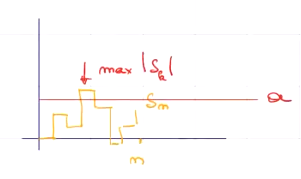
\includegraphics[width=0.6\linewidth]{screenshot017}
		\caption{The maximum of the random walk.}
		\label{fig:screenshot017}
	\end{figure}
	About this, we know that $\{S_{n}\}$ is a $\F$-martingale but in proving the Kolmogorov's inequaility we never talked about the martingale property! We could improve this inequality using the \emph{Doob's martingale inequality}. The problem is that we can prove very general inequalities that hold true for any \rv s but specifying more characteristic we can obtain stricter bounds. In this framework let's define 
	\begin{equation*}
		\begin{array}{l}
			M^{\star}_{n}=\max_{k\leq n}M_{k}\\
			m^{\star}_{n}=\min_{k\leq n}M_{k}\\
		\end{array}
	\end{equation*}
	as current maximum and current minimum of $M$.
	\begin{theorem}
		Take $M$ as a sub-martingale. For $b>0$ it holds:
		\begin{enumerate}
			\item $b\pr(M^{\star}_{n}\geq b)\leq\ev\left[M_{n}\indi_{\{M_{n}^{\star}\geq b\}}\right]\leq\ev\left[M_{n}^{+}\right]$;
			\item $b\pr(m^{\star}_{n}\leq-b)\leq-\ev M_{0}+\ev\left[M_{n}\indi_{\{m_{n}^{\star}\geq b\}}\right]\leq\ev M_{n}^{+}-\ev M_{0}$.
		\end{enumerate}
	\end{theorem}
	So we can further bound the result looking into the property of $M_{n}$.
	\begin{example}
		Now need to define the brownian motion (or Weiner process).
		\begin{definition}
			A real-valued stochastic process $B={(B_{t})}_{t\geq0}$ is called \emph{brownian motion} if:
			\begin{enumerate}
				\item the index set is $\R^{+}$;
				\item $B_{0}(\omega)=0$ for almost all $\omega$;
				\item $B_{t_{n}}-B_{t_{n-1}},\ldots,B_{t_{1}}-B_{t_{0}}$ are independent for $\every 0=t_{0}<t_1<\ldots<t_n<\infty$;
				\item $B_{t}-B_{s}\sim B_{t+b}-B_{s+b}$ for every $0\leq s<t<\infty\quad\every n>- s$;
				\item $B_{t}-B_{s}\sim N(0,t-s)$;
				\item $t\mapsto B_{t}(\omega)$ are continuous for every $\omega$.
			\end{enumerate}
		\end{definition}
		The brownian motion is in itself a martingale, but there is a class of martingales strictly related to it:
		\begin{equation*}
			M_{t}=\exp\left\{\lambda B_{t}-\frac{1}{2}\lambda^{2}t\right\},\qquad t\in\R^{+}.
		\end{equation*}
		Now we can get to the actual example: if $B$ is a brownian motion, we have 
		\begin{equation*}
			\pr(\sup_{0\leq t\leq\theta}B_{t}\geq b)\leq\exp\left\{-\frac{b^{2}}{s\theta}\right\}.
		\end{equation*}
		The sample paths of brownian motions are extremely irregular. We are asking with which probability the max of our process will be over $b$ at time $\theta$.
		\begin{figure}[H]
			\centering
			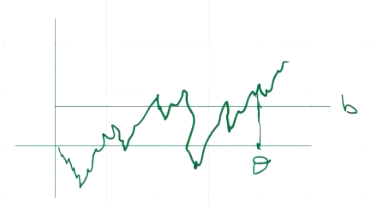
\includegraphics[width=0.6\linewidth]{screenshot018}
			\label{fig:screenshot018}
		\end{figure}
		I am basically asking if the maximum attained is above or below $b$.
		How can we use the Doob's inequality?
		\begin{fancyproof}
			Consider
			\begin{equation*}
				\pr(\sup B_{t}\geq b)=\pr(\sup e^{\lambda B_{t}}\geq e^{\lambda b})
			\end{equation*}
			and using Doob's inequality
			\begin{align*}
				\pr(\sup B_{t}\geq b)&=\pr(\sup e^{\lambda B_{t}}\geq e^{\lambda b})\\
				&\leq \frac{\overbrace{\ev\left[e^{\lambda B_{\theta}-\frac{\lambda^{2}}{2}\theta}\right]}^{\text{martingale}}}{e^{\lambda b}e^{-\frac{\lambda^{2}}{2}\theta}}\\
				&=e^{-\lambda b+\frac{\lambda^{2}}{2}\theta}\qquad\every\lambda>0
			\end{align*}
		\end{fancyproof}
	\end{example}
	\subsection{Predictable processes and Doob’s decomposition}
	\begin{definition}
		The process $F={(F_{n})}_{n\geq1}$ is \emph{$\F$-predictable} if $F_{0}\in\F_{0}$ and $\F_{n+1}\in\F_{n}$, for $\every n\in\N$.
	\end{definition}
	This means that the available information up to $n$ is ``enough'' to have a bet in the period $n+1$. Some predictable processes are:
	\begin{itemize}
		\item any deterministic processes;
		\item consider two stopping times $S,T$ of $\F$ and let $S\leq T$. Consider the \rv{} $V$ in $\F_{n}$. Then
		\[\begin{array}{c c c c}
			\color{DodgerBlue3}(1)&\color{DodgerBlue3}(2)&\color{DodgerBlue3}(3)&\color{DodgerBlue3}(4)\\
			V\indi_{(S,T]}&V\indi_{(S,\infty]}&\indi_{(S,T]}&\indi_{(0,T]}
		\end{array}\]
		are predictable processes.
		\begin{fancyproof}
			\begin{enumerate}
				\item[\color{DodgerBlue3}(2)] Consider $F=V\indi_{(S,\infty]}$, so that $F_{n}=\indi_{(S,\infty]}(n)$. Consider \begin{align*}
					F_{n+1}&=V\indi_{(S,\infty]}(n+1)\\
					&=V\indi_{\{S<n+1\}}\\
					&=V\indi_{\{S\leq n\}}\in\F_{n}
				\end{align*}
				so the process is $\F$-measurable and predictable.
				\item[\color{DodgerBlue4}(1)] Since we know by hypothesis that $S\leq T$ then $V\in\F_{S}\subset\F_{T}$. This means that $V\in\F_{T}$. Hence, of a consequence,
				\begin{equation*}
					V\indi_{(T,\infty]}-V\indi_{(S,\infty]}=V\indi_{(S,T]}
				\end{equation*}
				is predictable.
				\item[\color{DodgerBlue3}(3)] Take $V=1$.
				\item[\color{DodgerBlue3}(4)] Take $T=\infty$, $V=1$. $\indi_{(S,\infty]}$ is predictable. But then 
				\[\indi_{[0,S]}=\indi-\indi_{(S,\infty]}\]
				so it is predictable.
			\end{enumerate}
		\end{fancyproof}
	\end{itemize}
	\begin{theorem}
		\emph{Doob's decomposition}.\\
		$X$ is a stochastic process which is adapted to $\F$ and integrable. Then
		\begin{enumerate}
			\item it can be decomposed as 
			\[X_{n}=X_{0}+M_{n}+A_{n},\qquad n\in\N\]
			where:
			\begin{itemize}
				\item $M_{n}$ is a $\F$-martingale with $M_0=0$;
				\item $A_{n}$ is a predictable process with $A_0=0$.
			\end{itemize}
			\item The decomposition is unique up to equivalence.
			\item If $X_{n}$ is a sub-martingale then ${\{A_{n}\}}_{n\geq0}$ increasing, while if $X_{n}$ is a super-martingale then ${\{A_{n}\}}_{n\geq0}$ is decreasing.
		\end{enumerate}
	\end{theorem}
	\begin{fancyproof}
		Put $A_0=M_0=0$. Define $M$ and $A$ through their increments:
		\[ \begin{array}{l l}
			A_{n+1}-A_{n}&=\underbracket[0.3pt]{\ev\Big[X_{n+1}-X_{n}|\F_{n}\Big]}_{\F_{n}-\text{meas.}}\\
			M_{n+1}-M_{n}&=(X_{n+1}-X_{n})-(A_{n+1}-A_{n}).
		\end{array} \]
		If we look at these quantities we see that $A$ is predictable and $M$ is martingale. Imagine now there is another decomposition: let
		\[X=X_0+M'+A'\]
		be another decomposition. We must have
		\[\cancel{X_0}+M'+A'=\cancel{X_0}+M+A\iff A-A'=M-M'=B.\]
		Now $B$ is a process and it is predictable and martingale (because it is the difference between two martingales). Since $B$ is predictable \textit{and} a martingale we have
		\begin{align*}
			B_{n+1}-B_{n}&\underset{\mathclap{\text{\tiny predictable}}}{=}\ev[B_{n+1}-B_{n}|\F_{n}]\\
			&\underset{\mathclap{\text{\tiny martingale}}}{=}0\\
			&\implies B_{n+1}=B_{n}=B_0\;\as,A=A'\;\as,M=M'\as\\
		\end{align*}
		If $X$ is a sub-martingale then we have
		\[\ev[X_{n+1}-X_{n|\F_{n}}]\geq0\]
		and this means that we have $A_{n+1}\geq A_{n}$ is increasing.
	\end{fancyproof}
	\subsection{Doob’s stopping theorem}
	For a martingale we know
	\[\ev[X_{t}-X_{s}|\F_{s}]=0.\]
	The question is: is this true also if $s$ and $t$ are substituted by stopping times $S,T,S\leq T$?
	\begin{theorem}
		Let $M$ be adapted to $\F$. Then the following are equivalent:
		\begin{enumerate}[\circnum]
			\item $M$ is a submartingale;
			\item for every bounded stopping time $S\leq T$ the \rv s $M_{S}$ and $M_{T}$ are integrable and 
			\[\ev[M_{T}-M_{S}|\F_{S}]\geq0;\]
			\item for each pair of bounded stopping times the \rv s $M_{S}$ and $M_{T}$ are integrable and 
			\[\ev[M_{T}-M_{S}]\geq 0.\] 
		\end{enumerate}
	\end{theorem}
	\begin{remark}
		If $M$ is a martingale the theorem can be read in a different way:
		\begin{equation*}
			\ev M_{T}=\ev M_{S}=\ev M_{0}.
		\end{equation*}
		Previously, $\ev M_{n}=\ev M_{n-1}=\ev M_{0}$.
	\end{remark}
	\begin{fancyproof}
		To prove the theorem we need to show that from condition 1 follows 2 from which follows 3 from which follows 1.
		\begin{enumerate}
			\item[$1\to 2$] by hypothesis $M$ is a sub-martingale and our thesis is that if $S(\omega)<T(\omega)<n$ (because we asked for bounded times) then:
			\begin{enumerate}
				\item $M_{S}$ and $M_{T}$ are integrable;
				\item $\ev[M_{T}-M_{S}|\F_{S}]\geq0$.
			\end{enumerate}
			We know that $S$ and $T$ are bounded by $n$. Let $V$ be a positive bounded \rv{} and define $F=V\indi_{(S,T]}$ and use it in the discrete time integral:
			\[X_{n}=\underbrace{M_0F_0}_{X_0}+(M_1-M_0)\underbrace{F_1}_{\mathclap{V\indi_{\{1\in(S,T]\}}}}+\ldots+(M_{n}-M_{n-1})F_{n}\]
			So we have 
			\[X_{n}-X_{0}=V(M_{T}-M_{S})\]
			So $X_{n}$ is a sub-martingale. Take $V=1$ and $S=0$: now we have
			\begin{equation*}
				\begin{array}{c c c l}
					X_{n}&-&X_{0}&=M_{T}\\
					\downarrow&&\downarrow&\\
					\text{int.}&&\text{int.}&\implies M_{T}\text{ is integrable}.
				\end{array}
			\end{equation*}
			Now take $V=1$ and $T=n$ so that we get
			\begin{equation*}
				\begin{array}{c c c c l}
					X_{n}&-&X_{0}&=M_{n}&-M_{S}\\
					\downarrow&&\downarrow&\downarrow&\\
					\text{int.}&&\text{int.}&\text{int.}&\implies M_{S}\text{ is integrable}.
				\end{array}
			\end{equation*}
			We recall that $V\in\F_S$ and we use the defining property for $\ev(\cdot|\F_S)$. So we can write
			\begin{align*}
				\ev V\ev(M_{T}-M_{S}|\F_{S})&\underset{\mathclap{\text{def. prop.}}}{=}\ev V(M_{T}-M_{S})\\
				&\underset{\mathllap{\text{discr. time int.}}}{=}\ev[X_{n}-X_{0}]\\
				&\underset{\mathllap{\text{proved above}}}{\geq}0
			\end{align*}
			and this is true $\every V>0,V<b,V\in\F_{s}$. Hence
			\begin{equation*}
				\ev(M_{T}-M_{S}|\F_{S})\geq 0
			\end{equation*}
			So $1\to2$.
			\item[$2\to3$] We can use the tower rule. Take the expectation of point 2:
			\[\ev[\ev(M_{T}-M_{S}|\F_{S})]=\ev[M_{T}-M_{S}]\geq0.\]
			\item[$3\to1$] Let $3$ hold, so that $\ev[M_{T}-M_{S}]\geq0$. Choose $T=n$ and $S=0$. Then
			$M_{n}$ is integrable. Move to adaptness: this holds by hypothesis. Move to the martingale inequality:
			\begin{equation*}
				\ev[M_{n}-M_{m}|\F_{m}]\geq0.
			\end{equation*}
			Note that this is equivalent to prove 
			\begin{equation*}
				\ev\indi_H\ev[M_{n}-M_{m}|\F_{m}]\geq0\qquad H\in\F_{m},0\leq m\leq n.
			\end{equation*}
			Fix $H,m,n$ and define
			\begin{equation*}
				S(\omega)=m\qquad T(\omega)=n\indi_H(\omega)+m\indi_{\{\Omega\setminus H\}}(\omega)
			\end{equation*}
			The indicators are non-zero in complementary instances. Notice that:
			\begin{enumerate}
				\item $S$ is a fixed time so it is a stopping time;
				\item $S\leq T\leq n$ by definition of $S$ and $T$ because the indicators are non-zero in complementary instances;
				\item $T\geq S$ is a foretold time by $S=m$;
				\item $H\in\F_{S}$ by definition.
			\end{enumerate}
			So we can write $M_{T}-M_{S}=\indi_H(M_{n}-M_{m})$ where $M_{T}-M_{S}\geq0$ by hypothesis. This means that we have 
			\begin{equation*}
				\underbrace{\ev[\indi_{H}\ev(M_{n}-M_{m}|\F_{m})]}_{\ev[M_{n}-M_{m}|\F_{m}]\geq0}\geq0
			\end{equation*}
		\end{enumerate}
	\end{fancyproof}
	\subsection{Upcrossing inequality} 
	I believe that what is being asked is
	\begin{proposition}
		If $M$ is a sub-martingale with respect to its natural filtration then 
		\begin{equation*}
			(b-a)\ev U_{n}(a,b)\leq\ev\left[(M_{n}-a)^{+}-(M_{0}-a)^{+}\right].
		\end{equation*}
	\end{proposition}
	We wanted to find a bound for our profit, but our profit is a stochastic quantity: so it's only natural to think about the expectation to give a bound to the number of expected up/downcrossing.\\
	Observe that the number of upcrossings does not depend on the value of $T_0$ that we fix.
	\begin{fancyproof}
		Choose $a=0$. Consider hence the process $(M-a)^{+}$ that is sub-martingale (if $M$ is a sub-martingale). Take $M\geq 0$ and let 
		\begin{equation*}
			F_{n}-\sum_{k=1}^{\infty}\indi_{(S_{k},T_{k}]}(n)
		\end{equation*}
		and consider 
		\begin{equation*}
			X=\int F\dif M
		\end{equation*}
		like in our example. We know that $F$ is predictable since by definition $F_{k+1}\in\F_{k}$. Consider the expectation of the increment
		\begin{equation*}
			\ev[X_{k+1}-X_{k}|\F_{k}]=\ev\left[F_{k+1}(M_{k+1}-M_{k})|\F_{k}\right].
		\end{equation*}
		But since $F_{k+1}$ is predictable we can take it out the expectation:
		\begin{equation*}
			F_{k+1}\ev\left[M_{k+1}-M_{k}|\F_{k}\right].
		\end{equation*}
		But since $F_{k+1}$ is an indicator we know it is $\leq1$:
		\begin{equation*}
			\ev[X_{k+1}-X_{k}|\F_{k}]\leq\ev\left[M_{k+1}-M_{k}|\F_{k}\right].
		\end{equation*}
		Now take the expectation of both sides:
		\begin{equation*}
			\ev[X_{k+1}-X_{k}]\leq\ev\left[M_{k+1}-M_{k}\right].
		\end{equation*}
		If we sum these inequalities over $k$ we get:
		\begin{equation*}
			\ev\left[X_{n}-X_{0}\right]\leq\ev\left[M_{n}-M_{0}\right].
		\end{equation*}
		So we now get that
		\begin{equation*}
			bU_{n}(a,n)\leq\ev\left[X_{n}-X_{0}\right]\leq\ev\left[M_{n}-M_{0}\right]
		\end{equation*}
		but given that $a=0$ we get that
		\begin{equation*}
			bU_{n}(0,b)\leq\ev[M_{n}-M_{0}].
		\end{equation*}
		Clearly we have to take the positive part.
	\end{fancyproof}
	But I also found this
	\begin{proposition}
		Suppose that $\{X={X_{t}:t\in[0,\infty)}\}$ satisfies the basic assumptions with respect to the filtration $\F=\{\F_t:t\in[0,\infty)\}$ and let $a,b\in\R$ with $a<b$. Let $U_{t}=u_{t}(a,b,X)$ the random number of upcrossings of $[a,b]$ by $X$ up to time $t\in[0,\infty)$. 
		\begin{enumerate}[\circnum]
			\item if $X$ is a super-martingale relative to $\F$ then
			\begin{equation*}
				\ev(U_{t})\leq\frac{1}{b-a}\ev\left[(X_{t}-a)^{-}\right]\leq\frac{1}{b-a}\left[\ev(X_{t}^-)+|a|\right]\leq\frac{1}{b-a}\left[\ev(|X_{t}|)+|a|\right];
			\end{equation*}
			\item if $X$ is a sub-martingale relative to $\F$ then
			\begin{equation*}
				\ev(U_{t})\leq\frac{1}{b-a}\ev\left[(X_{t}-a)^{+}\right]\leq\frac{1}{b-a}\left[\ev(X_{t}^+)+|a|\right]\leq\frac{1}{b-a}\left[\ev(|X_{t}|)+|a|\right];
			\end{equation*}
		\end{enumerate}	
	\end{proposition}
	\subsection{Doob’s decomposition}
	\begin{theorem}
		\emph{Doob's decomposition}.\\
		$X$ is a stochastic process which is adapted to $\F$ and integrable. Then
		\begin{enumerate}
			\item it can be decomposed as 
			\[X_{n}=X_{0}+M_{n}+A_{n},\qquad n\in\N\]
			where:
			\begin{itemize}
				\item $M_{n}$ is a $\F$-martingale with $M_0=0$;
				\item $A_{n}$ is a predictable process with $A_0=0$.
			\end{itemize}
			\item The decomposition is unique up to equivalence.
			\item If $X_{n}$ is a sub-martingale then ${\{A_{n}\}}_{n\geq0}$ increasing, while if $X_{n}$ is a super-martingale then ${\{A_{n}\}}_{n\geq0}$ is decreasing.
		\end{enumerate}
	\end{theorem}
	\begin{fancyproof}
		Put $A_0=M_0=0$. Define $M$ and $A$ through their increments:
		\[ \begin{array}{l l}
			A_{n+1}-A_{n}&=\underbracket[0.3pt]{\ev\Big[X_{n+1}-X_{n}|\F_{n}\Big]}_{\F_{n}-\text{meas.}}\\
			M_{n+1}-M_{n}&=(X_{n+1}-X_{n})-(A_{n+1}-A_{n}).
		\end{array} \]
		If we look at these quantities we see that $A$ is predictable and $M$ is martingale. Imagine now there is another decomposition: let
		\[X=X_0+M'+A'\]
		be another decomposition. We must have
		\[\cancel{X_0}+M'+A'=\cancel{X_0}+M+A\iff A-A'=M-M'=B.\]
		Now $B$ is a process and it is predictable and martingale (because it is the difference between two martingales). Since $B$ is predictable \textit{and} a martingale we have
		\begin{align*}
			B_{n+1}-B_{n}&\underset{\mathclap{\text{\tiny predictable}}}{=}\ev[B_{n+1}-B_{n}|\F_{n}]\\
			&\underset{\mathclap{\text{\tiny martingale}}}{=}0\\
			&\implies B_{n+1}=B_{n}=B_0\;\as,A=A'\;\as,M=M'\as\\
		\end{align*}
		If $X$ is a sub-martingale then we have
		\[\ev[X_{n+1}-X_{n|\F_{n}}]\geq0\]
		and this means that we have $A_{n+1}\geq A_{n}$ is increasing.
	\end{fancyproof}
	\subsection{Stochastic integral in discrete time}
	Let us consider two real-valued processes $M={(M_{n})}_{n}$ and $F={(F_{n})}_{n}$ and let us define
	\[X_{n}=F_0M_{0}+(M_1-M_0)F_1+\ldots+(M_{n}-M_{n-1})F_n.\]
	We say that $\{X_{n}\}$ is the integral of $F$ with respect to $M$ and we write
	\[X_{n}=\int F \dif M\]
	where $\dif M$ is a random signed measure. Remember the Lebesgue-Stieltjes integral? Me neither, but as long as $M$ has bounded variation this is a Lebesgue-Stieltjes integral. So a little explanation is due since I actually never saw a Stieltjes integral.
	\begin{theorem}
		Consider $F$ bounded and predictable. Then if $M$ is a martingale then $X$ is a martingale; If $M$ is a sub(super)-martingale then $X$ is a sub(super)-martingale.
	\end{theorem}
	This means that... \emph{we can't beat the system!}
	\begin{flushright}
		\begin{tikzpicture}
			\calloutquote[width=4cm,position={(1,-1)},fill=Turquoise4!30,rounded corners]{I can beat something else though.}
		\end{tikzpicture}\hspace*{2.5cm}
	\end{flushright}
	\begin{example}
		Consider $M_{n}$ as the price of a share at time $n$ and $F_{n}$ as the number of shares owned during $(n-1,n]$. Our profit will be 
		\[(M_{n}-M_{n=1})F_{n}\]
		and our total profit $X_{n}$ gained during $(0,n]$ will be:
		\[X_{n}=X_{0}+\underbrace{\sum_{k=1}^{n}(M_{k}-M_{k-1})F_{k}}_{\mathclap{\text{discrete time integral}}}\]
		$F_{n}$ is based on the knowledge in $n-1$ so it is predictable. The process $M_{n}$ should be a martingale (otherwise if it is a sub/super-martingale everyone/no one will buy). So the total profit will also be a martingale! We can only choose our buying politics $F_{k}$, but there is no way to select a politics that will change a martingale in a super-martingale or sub-martingale.
	\end{example}
	Clearly this works in mean! 
	\begin{fancyproof}
		\begin{enumerate}
			\item	We have $M$ being a martingale and $F_0,F_1,\ldots,F_n\in\F_{n}$ as well as $M_0,M_1,\ldots,M_{n}\in\F_n$. Therefore $X_{n}\in\F_{n}$ and $X$ is adapted to $\F$.
			\item We need to check whether the discrete time integral is a martingale. We know by hypothesis that $F$ is bounded, so $F<b$ for some $b$. This implies
			\begin{equation*}
				|X_{n}|<b(|M_{0}|+|M_1+M_0|+\ldots+|M_n-M_{n-1}|)
			\end{equation*}
			Since $M$ is a martingale and it is integrable, we get that $X_n$ is bounded and integrable.
			\item Consider
			\begin{equation*}
				\ev[X_{n+1}-X_{n}|\F]=\ev[F_{n+1}(M_{n+1}-M_{n})|\F_n]
			\end{equation*}
			since all the terms cancel out and only the last ones survive. But $F_{n+1}\in\F_{n}$ so we can take it out of the expectation:
			\[F_{n}\underbrace{\ev[M_{n+1}-M_{n}|\F_{n}]}_{=0}=0.\]
		\end{enumerate}
	\end{fancyproof}
	\subsection{Stochastic integral and its application}
	Let us consider two real-valued processes $M={(M_{n})}_{n}$ and $F={(F_{n})}_{n}$ and let us define
	\[X_{n}=F_0M_{0}+(M_1-M_0)F_1+\ldots+(M_{n}-M_{n-1})F_n.\]
	We say that $\{X_{n}\}$ is the integral of $F$ with respect to $M$ and we write
	\[X_{n}=\int F \dif M\]
	where $\dif M$ is a random signed measure. Remember the Lebesgue-Stieltjes integral? Me neither, but as long as $M$ has bounded variation this is a Lebesgue-Stieltjes integral. So a little explanation is due since I actually never saw a Stieltjes integral.
	\begin{theorem}
		Consider $F$ bounded and predictable. Then if $M$ is a martingale then $X$ is a martingale; If $M$ is a sub(super)-martingale then $X$ is a sub(super)-martingale.
	\end{theorem}
	This means that... \emph{we can't beat the system!}
	\begin{flushright}
		\begin{tikzpicture}
			\calloutquote[width=4cm,position={(1,-1)},fill=Turquoise4!30,rounded corners]{I can beat something else though.}
		\end{tikzpicture}\hspace*{2.5cm}
	\end{flushright}
	\begin{example}
		Consider $M_{n}$ as the price of a share at time $n$ and $F_{n}$ as the number of shares owned during $(n-1,n]$. Our profit will be 
		\[(M_{n}-M_{n=1})F_{n}\]
		and our total profit $X_{n}$ gained during $(0,n]$ will be:
		\[X_{n}=X_{0}+\underbrace{\sum_{k=1}^{n}(M_{k}-M_{k-1})F_{k}}_{\mathclap{\text{discrete time integral}}}\]
		$F_{n}$ is based on the knowledge in $n-1$ so it is predictable. The process $M_{n}$ should be a martingale (otherwise if it is a sub/super-martingale everyone/no one will buy). So the total profit will also be a martingale! We can only choose our buying politics $F_{k}$, but there is no way to select a politics that will change a martingale in a super-martingale or sub-martingale.
	\end{example}
	Clearly this works in mean! 
	\begin{fancyproof}
		\begin{enumerate}
			\item	We have $M$ being a martingale and $F_0,F_1,\ldots,F_n\in\F_{n}$ as well as $M_0,M_1,\ldots,M_{n}\in\F_n$. Therefore $X_{n}\in\F_{n}$ and $X$ is adapted to $\F$.
			\item We need to check whether the discrete time integral is a martingale. We know by hypothesis that $F$ is bounded, so $F<b$ for some $b$. This implies
			\begin{equation*}
				|X_{n}|<b(|M_{0}|+|M_1+M_0|+\ldots+|M_n-M_{n-1}|)
			\end{equation*}
			Since $M$ is a martingale and it is integrable, we get that $X_n$ is bounded and integrable.
			\item Consider
			\begin{equation*}
				\ev[X_{n+1}-X_{n}|\F]=\ev[F_{n+1}(M_{n+1}-M_{n})|\F_n]
			\end{equation*}
			since all the terms cancel out and only the last ones survive. But $F_{n+1}\in\F_{n}$ so we can take it out of the expectation:
			\[F_{n}\underbrace{\ev[M_{n+1}-M_{n}|\F_{n}]}_{=0}=0.\]
		\end{enumerate}
	\end{fancyproof}
	and for the applications:\\
	\begin{definition}
		Define $M={(M_{n})}_{n\in\N}$ as a process and let $T$ be a random time with values on $\overline{\N}$. The process
		\[X_{n}(\omega)=M_{n\wedge T}(\omega)=\begin{cases}
			M_{n}(\omega)&n<T(\omega)\\
			M_{T}(\omega)&n>T(\omega)
		\end{cases}\]
		(where $n\wedge T$ is a truncated random time) is called \emph{$M$ stopped at $T$}.
	\end{definition}
	As a consequence $X$ is exactly the discrete time integral if $F=\indi_{[0,T]}$:
	\begin{equation*}
		X_{n}=\underbracket[0.6pt]{M_0F_0}_{0}+(M_{1}+M_{0})\indi_{[0,T]}(1)+\ldots+(M_{n}-M_{n-1})\indi_{[0,T]}(n).
	\end{equation*}
	The indicators only select the current time interval. If this is the case we can observe that $F_{[0,T]}$ is bounded, positive and predictable. Hence if $M$ is a martingale the theorem applies with this special choice of $M$ and we can write the result as a different theorem:
	\begin{theorem}
		Let $T$ be a stopping time and let $X$ be the process $M$ stopped at $T$. If $M$ is a martingale then so is $X$ (the same holds for sub-martingales and super-martingales).
	\end{theorem}
	So we cannot determine a policy based on stopping times that can change the nature of our martingale. In the remote case in which you are interested in this you can read Williams - Introduction to martingales. \\
	\subsection{Impossibility to win against the system: related theorems and examples}
	\begin{theorem}
		Consider $F$ bounded and predictable. Then if $M$ is a martingale then $X$ is a martingale; If $M$ is a sub(super)-martingale then $X$ is a sub(super)-martingale.
	\end{theorem}
	This means that... \emph{we can't beat the system!}
	\begin{flushright}
		\begin{tikzpicture}
			\calloutquote[width=4cm,position={(1,-1)},fill=Turquoise4!30,rounded corners]{I can beat something else though.}
		\end{tikzpicture}\hspace*{2.5cm}
	\end{flushright}
	\begin{example}
		Consider $M_{n}$ as the price of a share at time $n$ and $F_{n}$ as the number of shares owned during $(n-1,n]$. Our profit will be 
		\[(M_{n}-M_{n=1})F_{n}\]
		and our total profit $X_{n}$ gained during $(0,n]$ will be:
		\[X_{n}=X_{0}+\underbrace{\sum_{k=1}^{n}(M_{k}-M_{k-1})F_{k}}_{\mathclap{\text{discrete time integral}}}\]
		$F_{n}$ is based on the knowledge in $n-1$ so it is predictable. The process $M_{n}$ should be a martingale (otherwise if it is a sub/super-martingale everyone/no one will buy). So the total profit will also be a martingale! We can only choose our buying politics $F_{k}$, but there is no way to select a politics that will change a martingale in a super-martingale or sub-martingale.
	\end{example}
	Clearly this works in mean! 
	\begin{fancyproof}
		\begin{enumerate}
			\item	We have $M$ being a martingale and $F_0,F_1,\ldots,F_n\in\F_{n}$ as well as $M_0,M_1,\ldots,M_{n}\in\F_n$. Therefore $X_{n}\in\F_{n}$ and $X$ is adapted to $\F$.
			\item We need to check whether the discrete time integral is a martingale. We know by hypothesis that $F$ is bounded, so $F<b$ for some $b$. This implies
			\begin{equation*}
				|X_{n}|<b(|M_{0}|+|M_1+M_0|+\ldots+|M_n-M_{n-1}|)
			\end{equation*}
			Since $M$ is a martingale and it is integrable, we get that $X_n$ is bounded and integrable.
			\item Consider
			\begin{equation*}
				\ev[X_{n+1}-X_{n}|\F]=\ev[F_{n+1}(M_{n+1}-M_{n})|\F_n]
			\end{equation*}
			since all the terms cancel out and only the last ones survive. But $F_{n+1}\in\F_{n}$ so we can take it out of the expectation:
			\[F_{n}\underbrace{\ev[M_{n+1}-M_{n}|\F_{n}]}_{=0}=0.\]
		\end{enumerate}
	\end{fancyproof}
	We know that using a policy that it is predictable it is impossible to beat the system. Finance bros try to overcome this possibility using stopping times. If my policy is not only based on a predictable process but I add the randomness of the time in which I decide to sell or buy can I break the curse of martingales and make shareholders want to suck my dick? Well, it depends.
	\subsection{Predictable and adapted processes: definition and examples}
	\begin{definition}
		The process $F={(F_{n})}_{n\geq1}$ is \emph{$\F$-predictable} if $F_{0}\in\F_{0}$ and $\F_{n+1}\in\F_{n}$, for $\every n\in\N$.
	\end{definition}
	This means that the available information up to $n$ is ``enough'' to have a bet in the period $n+1$. Some predictable processes are:
	\begin{itemize}
		\item any deterministic processes;
		\item consider two stopping times $S,T$ of $\F$ and let $S\leq T$. Consider the \rv{} $V$ in $\F_{n}$. Then
		\[\begin{array}{c c c c}
			\color{DodgerBlue3}(1)&\color{DodgerBlue3}(2)&\color{DodgerBlue3}(3)&\color{DodgerBlue3}(4)\\
			V\indi_{(S,T]}&V\indi_{(S,\infty]}&\indi_{(S,T]}&\indi_{(0,T]}
		\end{array}\]
		are predictable processes.
		\begin{fancyproof}
			\begin{enumerate}
				\item[\color{DodgerBlue3}(2)] Consider $F=V\indi_{(S,\infty]}$, so that $F_{n}=\indi_{(S,\infty]}(n)$. Consider \begin{align*}
					F_{n+1}&=V\indi_{(S,\infty]}(n+1)\\
					&=V\indi_{\{S<n+1\}}\\
					&=V\indi_{\{S\leq n\}}\in\F_{n}
				\end{align*}
				so the process is $\F$-measurable and predictable.
				\item[\color{DodgerBlue4}(1)] Since we know by hypothesis that $S\leq T$ then $V\in\F_{S}\subset\F_{T}$. This means that $V\in\F_{T}$. Hence, of a consequence,
				\begin{equation*}
					V\indi_{(T,\infty]}-V\indi_{(S,\infty]}=V\indi_{(S,T]}
				\end{equation*}
				is predictable.
				\item[\color{DodgerBlue3}(3)] Take $V=1$.
				\item[\color{DodgerBlue3}(4)] Take $T=\infty$, $V=1$. $\indi_{(S,\infty]}$ is predictable. But then 
				\[\indi_{[0,S]}=\indi-\indi_{(S,\infty]}\]
				so it is predictable.
			\end{enumerate}
		\end{fancyproof}
	\end{itemize} 
	Example of adapted process:
	\begin{example}
		This is called ``the secretary problem'': in this case we must start from the filtration and then understand the problem.
		Here i have $N$ candidates for a position; a candidate disregarded after the interview is lost. The interviewer wants to hire exactly 1 candidate and each candidate has different abilities and the interviewer knows only the relative ability of those already interviewed so far. Our goal is to maximizing the probability of hiring the best one. We have three questions:
		\begin{enumerate}
			\item what is $\Omega$?
			\item what is the filtration $\F$ for this experiment?
			\item what process should we use?
		\end{enumerate}
		In this case $\Omega=N!$ permutations of the ranking of the candidates (the order in which they show up) and the filtration is the information earned from interview up to time $t$ (that is the ranking of the candidates up to time $t$). But what is the process that I should use? Consider the sequence
		\[V_1,V_2,\ldots\qquad{\{V_i\}}_{i\geq 1}\]
		with $V_i=1$ if and only if the best candidate is the $i$-th candidate and $V_i=0$ otherwise. Could this process ${\{V_i\}}_{i\geq 1}$ be used? No, because $V$ is not adapted to $\F$... because to understand if $i$-th candidate is te best we need to compare it to the other candidates, including the ones that didn't show up yet! But then how can we get an adapted process? Let us consider the expectation
		\[U_n=\ev\left[V_n|\F_n\right]\]
		What do we know about the measurability of $U_n$? We know that it is for sure $\F_n$-measurable. This trick gives us a simple way to build an adapted process. So now we will have:
		$U_n=
		0$ if the candidate is not the best up to $n$ and $U_n=1$ otherwise. More specifically, we will have
		\begin{align*}
			U_n&=1\cdot\substack{\text{proability that the best candidate}\\\text{is among the first $n$}}+0\cdot\substack{\text{proability that the best candidate}\\\text{is not among the first $n$}}\\
			&=1\cdot\frac{n}{N}+0\cdot\frac{N-n}{N}.\\
			&=\frac{n}{N}
		\end{align*}
		This is a quantity that I can measure and it is therefore adapted.\par
	\end{example}
	\subsection{Poisson process and its martingale property}
	Consider $\R_+$ as our index set. $\F$ is our filtration and we consider the counting process $N={(N_{t})}_{y\geq0}$: this counts the number of events up to time $t$, it has unit jumps and any path starts from 0 so that $N_{0}(\omega)=0$, it is increasing and it is right continuous.
	\begin{definition}
		The counting process $N$ is said to be a \emph{Poisson process} with rate $\lambda$ with respect to $\F$ if it is adapted to $\F$ and
		\[\ev[f(N_{t+s}-N_s)|\F_s]=\sum_{k=0}^{\infty}e^{-\lambda t}\frac{(\lambda t)^{k}}{k!}f(k)\qquad\every s,t\in\R_+,\every\text{positive }f\mapsto\N.\]
	\end{definition}
	\begin{theorem}
		Let $N$ be a counting process. It is a Poisson process with rate $\lambda$ with respect to $\F$ \ifonly{}:
		\begin{equation*}
			M_{t}=N_{t}-\lambda t
		\end{equation*}
		is a $\F$-martingale.
	\end{theorem}
	We only prove that $M_t$ is a martingale if $N_{t}$ is Poisson.
	\begin{fancyproof}
		We know that 
		\begin{align*}
			\ev[M_{t}|\F_{s}]&=\ev[M_{t}-M_{s}+M_{s}|\F_{s}]\\
			&=\ev[M_{t}-M_{s}|\F_{s}]+M_{s}\\
			&=\ev[M_{t}-M_{s}]+M_{s}\\
			&=\ev[N_{t}-N_{s}+\lambda t+\lambda s]+M_{s}\\
			&=\underbrace{\ev[N_{t}-N_{s}]}_{\cancel{\lambda (t-s)}}-\cancel{\lambda (t-s)}+M_{s}\\
			&=M_{s}
		\end{align*}
	\end{fancyproof}
	\subsection{Stopped processes and their properties}
	\begin{example}
		Some stopping times:
		\begin{enumerate}[\circnum]
			\item The first time that $X(\omega)\in H\in\Omega$;
			\[T(\omega)=\begin{cases}
				\inf \left\{n\in\N:X_n(\omega)\in H\right\}&\\
				+\infty&\text{if $X_n(\omega)\notin H\;\every n$}
			\end{cases}\]
			So
			\[\left\{T\leq n\right\}=\bigcup_{k=0}^{n}\left\{X_k\in H\right\}.\]
			\item Consider i.i.d. \rv{}s 
			$X_1,X_2,\ldots$. Consider the probabilities
			\[\pr(X_i=1)=\pr(X_i=-1)=\frac{1}{2}\]
			and the random walk
			\[S_n=\sum_{1}^{n}X_i.\]
			Let's define 
			\[T_1=\begin{cases}
				\min\left\{n<50:S_n=3\right\}\\
				50 &\text{otherwise}.
			\end{cases}\]
			This is a stopping time because I can write $\left\{T_1\leq n\right\}$ as $$\underbracket[0.6pt]{\bigcup_{k=1}^{n}\underbracket[0.6pt]{\left\{S_k=3\right\}}_{\text{$\F_k$-measurable}}}_{\mathclap{\text{$\F_n$-measurbale}}}\qquad n<50.$$
			Moreover for $n=50$ we have $T_{1}\in\F_{50}$.
			\item Starting from the previously deifned random walk, consider the quantity 
			\[M_n=\min(S_1,\ldots,S_n)\]
			And the random time
			\[T_2=\min\left\{n:S_n\geq M_m+2\right\}\]
			is a stoppimg time. On the contrary, 
			\[T_3=\begin{cases}
				\max\left\{n<50:S_n=7\right\}&\text{if not empty}\\
				50 &\text{otherwise}
			\end{cases}\]
			is not a stopping time. Why? Because I have to wait until $n=50$ to answer the question. 
		\end{enumerate}
	\end{example}
	
	Consider the random times on $\R_+$
	\[0<T_1<T_2<\ldots\]
	With $\lim_{n\to\infty}T_n=+\infty$. Define the process $\left\{N_t\right\}$ as 
	\[N_t:=\sum\indi_{[0,t]}(T_n).\]
	This is called \emph{counting process}. It is a basic count of the number of events happened up to time $n$.
	$N_{t}$ is increasing, right continuous and incresases by unitary jumps. Moreover, $N_0=0$, $N_t<\infty$ for $t\in\R_+$. Of course $\lim_{t\to\infty}N_t=\infty$. Counting processes generate their natural filtration $\F$.
	
	Some problems require to stop the observation at a stopping time (because we don't care anymore\footnote{Assuming we ever did.})... So we don't actually need the whole knowledge of the complete filtration $\F={\left(\F_t\right)}_{t\geq 0}$. The problem is that as we said before the stopping time is a random time. So what we need is the \textit{information known up to time $T$} $\F_T$, basically the $\sigma$-field that is the filtration at time $T$. 
	\begin{example}
		\emph{Truncated stopping time}: let $T$ be a stopping time (for example, the time at which we sell certain shares) and that we want a finite horizon for this decision. In this case the quantity of interest is
		\begin{equation*}
			S=T\wedge n=\min\{T,n\}
		\end{equation*}
		where $n$ could be some sort of time horizon.\\
		Imagine that two cyclists participate to a race. Their children will have their snack when both the parents will arrive to the finish line. How long will the children wait for their snack?
		We can think about the following stopping times:
		\[ 	\begin{array}{l l}
			T: & \text{time employed by the first cyclist}\\
			S: & \text{time employed by the second cyclist}\\
			U: &\max\{S,T\}.
			
		\end{array} \]
		The waiting time for the children will be $U$.
	\end{example}
	\subsection{Important inequalities for sub-martingales}
	The problem is that we can prove very general inequalities that hold true for any \rv s but specifying more characteristic we can obtain stricter bounds. In this framework let's define 
	\begin{equation*}
		\begin{array}{l}
			M^{\star}_{n}=\max_{k\leq n}M_{k}\\
			m^{\star}_{n}=\min_{k\leq n}M_{k}\\
		\end{array}
	\end{equation*}
	as current maximum and current minimum of $M$.
	\begin{theorem}
		Take $M$ as a sub-martingale. For $b>0$ it holds:
		\begin{enumerate}
			\item $b\pr(M^{\star}_{n}\geq b)\leq\ev\left[M_{n}\indi_{\{M_{n}^{\star}\geq b\}}\right]\leq\ev\left[M_{n}^{+}\right]$;
			\item $b\pr(m^{\star}_{n}\leq-b)\leq-\ev M_{0}+\ev\left[M_{n}\indi_{\{m_{n}^{\star}\geq b\}}\right]\leq\ev M_{n}^{+}-\ev M_{0}$.
		\end{enumerate}
	\end{theorem}
	So we can further bound the result looking into the property of $M_{n}$.
	\begin{fancyproof}
		We introduce 2 stopping times: 
		\begin{equation*}
			\begin{array}{l l}
				T&=\inf\{n\geq0:M_{n}\geq b\}\\
				S&=\inf\{n\geq0:M_{n}\leq-b\}.
			\end{array}
		\end{equation*}
		\begin{figure}[H]
			\centering
			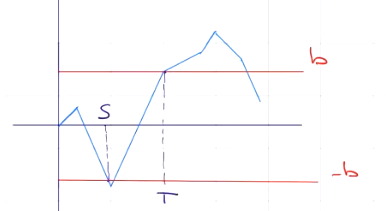
\includegraphics[width=0.6\linewidth]{screenshot019}
			\label{fig:screenshot019}
		\end{figure}
		Consider the current maximum and minimum above the level $b$:
		\begin{equation*}
			\{M^{\star}_{n}\geq b\}=\{T\leq n\}\qquad	\{m^{\star}_{n}<-b\}=\{S\leq n\}.
		\end{equation*}
		Fix $b$ and $n$. When $\{T\leq n\}$ we have
		\begin{align*}
			M_{T\wedge n}=M_{T}\geq b.
		\end{align*}
		Multiply by $\indi_{\{T\leq n\}}$:
		\begin{equation*}
			b\indi_{\{T\leq n\}}\leq M_{T\wedge m}\indi_{\{T\leq n\}}.
		\end{equation*}
		Using Doob's stopping theorem we know that 
		\begin{equation*}
			\ev\left[M_{T}-M_{S}|\F_{S}\right]\geq0
		\end{equation*}
		and using $S=T\wedge n$ and $T=n$ we obtain
		\begin{equation*}
			\ev\left[M_{n}|\F_{T\wedge n}\right]>M_{T\wedge n}.
		\end{equation*}
		So summing it all up:
		\begin{align*}
			b\indi_{\{T\leq n\}}&\leq M_{T\wedge m}\indi_{\{T\leq n\}}\\
			&\leq\indi_{\{T\leq n\}}\ev\left[M_{n}|\F_{T\wedge n}\right]\\
			&\ev\left[M_{n}\indi_{\{T\leq n\}}|\F_{T\wedge n}\right].
		\end{align*}
		Now take the expectation:
		\begin{align*}
			b\pr(T\leq n)&=b\pr(M^{\star}_{n}\geq b)\\
			&\leq\underbrace{\ev\left[M_{n}\indi_{\{T\leq n\}}\right]}_{\mathclap{\ev\left[M_{n}\indi_{\{M_{n}^{\star}\geq b\}}\right]}}\\
			&\leq\ev(M^{+}_{n}).
		\end{align*}
		For the minimum we work on $\{S\leq n\}$ and we get 
		\begin{align*}
			M_{S\wedge n}&=M_{S}\indi_{\{S\leq n\}}+M_{S}\indi_{\{S>n\}}\\
			&\leq-b\indi_{\{S\leq n\}}+M_{n}\indi_{S\geq n}.
		\end{align*}
		Now take the expectation:
		\begin{equation*}
			\ev M_{S\wedge n}\leq-b\pr(m^{\star}_{n}\leq-b)+\ev\left[M_{n}\indi_{\{S>n\}}\right].
		\end{equation*}
		So that we get
		\begin{equation*}
			\pr(m^{\star}_{n}\leq-b)\leq-\ev M_{S\wedge n}+\ev[M_{n}\indi_{\{S>n\}}].
		\end{equation*}
		Now use Doob's stopping theorem with $T=0$ and $S=S\wedge n$ so that $\ev M_{0}\leq\ev M_{\{S\wedge n\}}$. This gets us our result:
		\begin{align*}
			b\pr(m^{\star}_{n}-b)&\leq-\ev M_{0}+\ev\left[M_{n}\indi_{\{m_{n}^{\star}\}}\right]\\
			&\leq\ev M^{+}_{n}-\ev M_{0}.
		\end{align*}
	\end{fancyproof}
	\subsection{Convergence theorems for sub-martingales}
	\begin{theorem}
		Let $X$ be a sub-martingale. If (and note that is a sufficient condition)
		\begin{equation*}
			\sup_{n}\ev X_{n}^{+}<\infty
		\end{equation*}
		Then
		\begin{enumerate}
			\item $\{X_{n}\}$ converges $\as$;
			\item $\{X_{n}\}$ converges to an integrable \rv.
		\end{enumerate}
	\end{theorem}
	\begin{fancyproof}
		We prove the theorem by contradiction. Pick an outcome $\omega$ and suppose that $\{X_{n}(\omega)\}$ is a numerical sequence that has not a limit. But if it doesn't have a limit, then 
		\[\exists\inf\lim\neq\sup\lim\qquad\inf\lim<\sup\lim.\]
		So there exist at least 2 rationals $a<b$ such that
		\begin{equation*}
			\inf\lim<a<b<\sup\lim.
		\end{equation*}
		The sequence $\{X_{n}(\omega)\}$ crosses $(a,b)$ $\infty$ many times. Now take the union over rational $a$ and $b$, $a<b$ of the sets
		\begin{equation*}
			\{U(a,b)=\infty\}
		\end{equation*}
		with $U(a,b)=\lim_{n\to\infty}U_{n}(a,b)$. Our aim is now to show that $U(a,b)\leq\infty$ almost surely to get a contradiction.\\
		Fix $a,b$. We know that $U_{n}(a,b)$ is increasing with $n$. Now consider
		\begin{align*}
			(b-a)\ev U(a,b)&=(b-a)\ev\lim U_{n}(a,b)\\
			&\underset{\mathclap{\text{monotone conv.}}}{=}(b-a)\lim\ev U_{n}(a,b)\\
			&\underset{\mathclap{\text{upcross inequalities}}}{\leq}\sup\ev(X_n-a)^{+}\\
			&\leq \sup\ev X_{n}^{+}+|a|.
		\end{align*}
		So this means that $\ev U(a,b)<\infty$. But this is a contradiction, so it exists a limit $X_{n}=X_{\infty}\as$.\\
		Now consider the second part of the theorem:
		\begin{align*}
			\ev|X_{\infty}|&=\ev\lim\inf|X_{n}|\\
			&\underset{\mathclap{\text{Fatou's lemma}}}{\leq}\lim\inf\ev|X_{n}|\\
			&\leq 2\sup\ev X_{n}^{+}-\ev X_{0}\leq\infty
		\end{align*}
		so the limit is integrable.
	\end{fancyproof}
	\subsection{Uniform integrability and its consequences on convergence of martingales}
	We will need:
	\begin{enumerate}
		\item a collection $\mathcal{K}$ of real \rv s is said to be uniformly integrable if 
		\begin{equation*}
			k(b)=\sup_{X\in\mathcal{K}}\ev|X|\indi_{\{X>b\}}\xrightarrow[b\to\infty]{}0.
		\end{equation*}
		\item If $\mathcal{K}$ is dominated by an integrable \rv{} $Z$ then it is uniformly integrable.
		\item uniform integrability implies $L^{1}$-boundedness but not the converse.
		\item If $\mathcal{K}$ is $L^{p}$-bounded for some $p>1$ then it is uniformly integrable.
	\end{enumerate}
	\begin{lemma}
		Let $Z$ be an integrable \rv{}. Then
		\begin{equation*}
			\mathcal{K}=\left\{X:X=\ev(Z|\G)\right\}
		\end{equation*}
		for some sub-\sa{} $\G$ of $\HS$ is uniformly integrable.
	\end{lemma}
	\begin{proposition}
		Let $Z$ be an integrable \rv{}. Define 
		\begin{equation*}
			X_{t}=\ev(Z|\F_{t})\qquad t\in\T.
		\end{equation*}
		This means that $\{X_{t}\}$ is a uniformly integrable $\F$-martingale.
	\end{proposition}
	\begin{theorem}
		Let $\{X_{n}\}$ be a sequence of real-valued \rv s. The following are equivalent:
		\begin{enumerate}
			\item it converges in $L^{1}$;
			\item it converges in probability and it is uniformly integrable.
		\end{enumerate}
	\end{theorem}
	We can now prove the theorem about the convergence of sub-martingales.
	\begin{theorem}
		Let $X$ be a sub-martingale. We have that $X$ converges almost surely and in $L^{1}$ \ifonly{} it is uniformly integrable. Moreover, if it is so, setting 
		\begin{equation*}
			X_{\infty}=\lim X_{n}
		\end{equation*}
		extends $X$ to a sub-martingale
		\begin{equation*}
			\xbar={(X_{n})}_{n\in\overline{\N}}.
		\end{equation*}
	\end{theorem}
	We only prove the first part of the theorem.
	\begin{fancyproof}
		\emph{Necessity}. If $X$ converges in $L^{1}$ by the theorem above it is uniformly integrable.\\
		\emph{Sufficiency}. If $X$ is uniformly integral then it is $L^{1}$-bounded for the property above. So our previous theorem holds and the martingale converges almost surely with $X_{\infty}$ integrable. Furthermore, for the property above, it also converges in $L^{1}$.
	\end{fancyproof}
	\subsection{Features of the sample paths of a submartingale (or martingale)}
	\begin{remark}
		If $M$ is a martingale then $|M|^{p}$ is a sub-martingale for $p\geq1$. If $M_{n}\in\lp\every n$ we can apply Doob's inequality.
	\end{remark}
	\begin{corollary}
		If $M$ is martingale in $\lp$ for some $p\geq 1$ then for $b>0$ we have that
		\begin{equation*}
			b^{p}\pr(\max_{k\leq n}|M_{k}|>b)\leq\ev|M_{n}|^{p}.
		\end{equation*}
	\end{corollary}
	There are also other bounds:
	\begin{itemize}
		\item $b\pr(\max_{k\leq n}|M_{k}>b)\leq 2\ev M_{n}^{+}-3M_{0}$;
		\item \emph{Doob's norm inequality}: if $M$ is a martingale in $\lp,p\geq 1$ and $q$ is the exponent conjugate to $p$ ($\frac{1}{p}+\frac{1}{q}=1$) then
		\begin{equation*}
			\ev\max_{  k\leq n}|M_{k}|^{p}\leq q^{p}\ev|M_{n}|^{p}.
		\end{equation*}
		\item  Consider $L^{2}$-bounded martingales characterized by final coordinate $X$ with $\var X=\sigma^{2}$ (that is I am fixing the variance of the last value I consider). We want to assess the variability of this process.
		\begin{theorem}
			\emph{Dubin \& Schwartz 1998}: it holds
			\begin{enumerate}
				\item $\ev\left[\max_{0\leq T\leq t}M_{T}\right]\leq\sigma$;
				\item $\ev\left[\max_{0\leq T\leq t}|M_{T}|\right]\leq\sigma\sqrt{2}$.
			\end{enumerate}
			Moreover, there exist suitable martingales for which this bound is attained and is scrict.
		\end{theorem}
	\end{itemize}
	\subsection{Uniform integrability and its role in convergence problems}
	\begin{theorem}
		A process $M={(M_{n})}_{n\in\N}$ is a uniformly integrable martingale \ifonly{} for some integrable \rv{} $Z$
		\begin{equation}
			M_{n}=\ev\left[Z|\F_{n}\right]\qquad n\in\N.\tag{$\bullet$}\label{AAAA}
		\end{equation}
		If so it converges almost surely and in $L^{1}$ to the integrable \rv
		\begin{equation*}
			M_{\infty}=\ev[Z|\F_{\infty}].
		\end{equation*}
	\end{theorem}
	\begin{corollary}
		For every integrable \rv{} $Z$ we have
		\begin{equation*}
			\ev(Z|\F_{n})\convas\xrightarrow[]{L^{1}}\ev(Z|\F_{\infty}).
		\end{equation*}
	\end{corollary}
	\begin{theorem}
		Let $Z$ be an integrable \rv{} and let 
		\begin{equation*}
			M_{n}=\ev(Z|\F_{n})_{n\in\overline{\N}}.
		\end{equation*}
		For every stopping time $T$ define
		\begin{equation*}
			M_{T}=\ev[Z|\F_{T}]
		\end{equation*}
		and for arbitrary stopping times $S$ and $T$ we get
		\begin{equation*}
			\ev[M_{T}|\F_{S}]=M_{S\wedge T}.
		\end{equation*}
	\end{theorem}
	This lets us rethink Doob's theorem.
	\begin{theorem}
		If $S$ and $T$ are arbitrary stopping times such that $S\leq T$ then
		\begin{equation*}
			\ev[M_{T}|\F_{S}]=M_{S}
		\end{equation*}
		for an uniformly integrable martingale.
	\end{theorem}
	The dominated convergence theorem requires adaptness. 
	\begin{theorem}
		\emph{Hunt's dominated convergence theorem}.\\
		Let $\{X_{n}\}$ be dominated by an integrable \rv{} and suppose that exists
		\begin{equation*}
			X_{\infty}=\lim X_{n}
		\end{equation*}
		So ${(\ev_{n}X_{n})}_{n}$ converges to $\ev X_{\infty}$ almost surely and in $L^{1}$.
	\end{theorem}
	\subsection{Stopped martingales}
	\begin{definition}
		Define $M={(M_{n})}_{n\in\N}$ as a process and let $T$ be a random time with values on $\overline{\N}$. The process
		\[X_{n}(\omega)=M_{n\wedge T}(\omega)=\begin{cases}
			M_{n}(\omega)&n<T(\omega)\\
			M_{T}(\omega)&n>T(\omega)
		\end{cases}\]
		(where $n\wedge T$ is a truncated random time) is called \emph{$M$ stopped at $T$}.
	\end{definition}
	As a consequence $X$ is exactly the discrete time integral if $F=\indi_{[0,T]}$:
	\begin{equation*}
		X_{n}=\underbracket[0.6pt]{M_0F_0}_{0}+(M_{1}+M_{0})\indi_{[0,T]}(1)+\ldots+(M_{n}-M_{n-1})\indi_{[0,T]}(n).
	\end{equation*}
	The indicators only select the current time interval. If this is the case we can observe that $F_{[0,T]}$ is bounded, positive and predictable. Hence if $M$ is a martingale the theorem applies with this special choice of $M$ and we can write the result as a different theorem:
	\begin{theorem}
		Let $T$ be a stopping time and let $X$ be the process $M$ stopped at $T$. If $M$ is a martingale then so is $X$ (the same holds for sub-martingales and super-martingales).
	\end{theorem}
	So we cannot determine a policy based on stopping times that can change the nature of our martingale. In the remote case in which you are interested in this you can read Williams - Introduction to martingales. \\
	A further theorem about this is \emph{Doob's stopping theorem}. For a martingale we know
	\[\ev[X_{t}-X_{s}|\F_{s}]=0.\]
	The question is: is this true also if $s$ and $t$ are substituted by stopping times $S,T,S\leq T$?
	\begin{theorem}
		Let $M$ be adapted to $\F$. Then the following are equivalent:
		\begin{enumerate}[\circnum]
			\item $M$ is a submartingale;
			\item for every bounded stopping time $S\leq T$ the \rv s $M_{S}$ and $M_{T}$ are integrable and 
			\[\ev[M_{T}-M_{S}|\F_{S}]\geq0;\]
			\item for each pair of bounded stopping times the \rv s $M_{S}$ and $M_{T}$ are integrable and 
			\[\ev[M_{T}-M_{S}]\geq 0.\] 
		\end{enumerate}
	\end{theorem}
	\begin{remark}
		If $M$ is a martingale the theorem can be read in a different way:
		\begin{equation*}
			\ev M_{T}=\ev M_{S}=\ev M_{0}.
		\end{equation*}
		Previously, $\ev M_{n}=\ev M_{n-1}=\ev M_{0}$.
	\end{remark}
\end{document}